% ITRI626 practical project report -- electronic-component image classification with four model families.
% Build: see README.md ("ITRI626 submission") or docs/itri626_report/RUBRIC_CHECKLIST.md.
% Tables and result-number macros are generated by make_tables.py from committed result files.
\documentclass[11pt,a4paper]{article}

\usepackage[T1]{fontenc}
\usepackage[utf8]{inputenc}
% Text: Charter (XCharter) with matching maths; Inconsolata (zi4) for code and file paths
\usepackage{XCharter}
\usepackage[xcharter]{newtxmath}
\usepackage[varqu,scaled=0.95]{zi4}
\usepackage[a4paper,margin=2.5cm]{geometry}
\usepackage[tracking=true]{microtype}
\SetTracking{encoding=*,shape=sc}{40}
\usepackage{graphicx}
\usepackage{booktabs}
\usepackage{array}
\usepackage{tabularx}
\usepackage{longtable}
\usepackage{multirow}
\usepackage{amsmath}
\usepackage{siunitx}
\usepackage{xcolor}
% model colours (Okabe--Ito), identical to the figures: A orange, B blue, C bluish green
\definecolor{mA}{HTML}{E69F00}\definecolor{mB}{HTML}{0072B2}\definecolor{mC}{HTML}{009E73}
\definecolor{mD}{HTML}{882255}
\definecolor{accent}{HTML}{1F3A5F}
\usepackage{xspace}
\xspaceaddexceptions{\,\%}
\usepackage{enumitem}
\usepackage{caption}
\usepackage{subcaption}
\usepackage{float}
\usepackage{needspace}
\usepackage{flafter}
\usepackage{placeins}
\usepackage[skip=4pt plus 1pt]{parskip}
\usepackage{titlesec}
\titleformat*{\section}{\Large\bfseries\color{accent}}
\titleformat*{\subsection}{\large\bfseries\color{accent}}
\titlespacing*{\section}{0pt}{2.2ex plus 1ex minus .2ex}{1.0ex plus .2ex}
\titlespacing*{\subsection}{0pt}{1.8ex plus 1ex minus .2ex}{0.6ex plus .1ex}
\usepackage{fancyhdr}
\usepackage[numbers,square,sort&compress]{natbib}
\usepackage{url}
\usepackage[colorlinks,linkcolor=accent,citecolor=accent,urlcolor=accent,bookmarksnumbered,
  pdftitle={Recognising electronic components in web photographs},
  pdfauthor={ITRI626 group},
  pdfsubject={ITRI626 practical project report}]{hyperref}
\usepackage[nameinlink,capitalise,noabbrev]{cleveref}

\graphicspath{{../../results/itri626/figures/}}
\sisetup{group-separator={,},group-minimum-digits=4,group-digits=integer,detect-weight,mode=text}
\captionsetup{font=small,labelfont={bf,color=accent},margin=0pt}
\setlist{itemsep=1pt,topsep=3pt,parsep=0pt}
\newcolumntype{Y}{>{\raggedright\arraybackslash}X}
\newcolumntype{V}{!{\color{black!35}\vrule width 0.3pt}}
\setlength{\emergencystretch}{1.5em}
\widowpenalty=10000 \clubpenalty=10000 \displaywidowpenalty=10000
\setlength{\textfloatsep}{14pt plus 2pt minus 4pt}\setlength{\floatsep}{10pt plus 2pt minus 2pt}
\renewcommand{\floatpagefraction}{0.60}
\renewcommand{\topfraction}{0.90}
\renewcommand{\textfraction}{0.08}
% file paths and URLs: break only at / _ - . and in a slightly smaller mono font
\def\UrlBreaks{\do\/\do\_\do\-\do\.}
\Urlmuskip=0mu plus 1mu
\makeatletter
\newcommand{\relsmall}{\fontsize{\fpeval{0.92*\f@size}}{\f@baselineskip}\selectfont}% 92% of the current size
\makeatother
\renewcommand{\UrlFont}{\ttfamily\relsmall}
\newcommand{\cls}[1]{#1}
\newcommand{\mA}{model~A\xspace}
\newcommand{\mB}{model~B\xspace}
\newcommand{\mC}{model~C\xspace}
\newcommand{\MA}{Model~A\xspace}
\newcommand{\MB}{Model~B\xspace}
\newcommand{\MC}{Model~C\xspace}
\newcommand{\mD}{model~D\xspace}\newcommand{\MD}{Model~D\xspace}
% small square in a model's figure colour, used before model names in tables
\newcommand{\msq}[1]{\textcolor{m#1}{\rule{0.75ex}{0.75ex}}\,}
% running header (the title page stays plain)
\pagestyle{fancy}\fancyhf{}
\fancyhead[L]{\small\color{black!60}ITRI626 \textperiodcentered{} Electronic-component classification}
\fancyhead[R]{\small\color{black!60}\nouppercase{\rightmark}}
\fancyfoot[C]{\small\thepage}
\renewcommand{\headrulewidth}{0.3pt}\setlength{\headheight}{14pt}
\renewcommand{\sectionmark}[1]{\markboth{\thesection\quad #1}{\thesection\quad #1}}
\renewcommand{\subsectionmark}[1]{}

% generated by docs/itri626_report/make_tables.py -- do not edit by hand
\newcommand{\nRaw}{3,530\xspace} % data/v2/leakage_report.json counts.raw_files
\newcommand{\nUnique}{2,943\xspace} % data/v2/leakage_report.json counts.unique_sha256
\newcommand{\nDupGroups}{533\xspace} % data/v2/leakage_report.json counts.exact_dup_groups
\newcommand{\nDupRedundant}{587\xspace} % data/v2/leakage_report.json counts.exact_dup_redundant_files
\newcommand{\nConflictGroups}{13\xspace} % data/v2/leakage_report.json counts.exact_dup_conflicting_label_groups
\newcommand{\nConflictFiles}{27\xspace} % data/v2/splits/split_summary.csv TOTAL.excluded_conflict_files
\newcommand{\nCorrupt}{0\xspace} % leakage_report unique_sha256 - decoded_unique
\newcommand{\nRows}{2,930\xspace} % data/v2/leakage_report.json counts.rows
\newcommand{\nClusters}{2,787\xspace} % data/v2/leakage_report.json counts.clusters
\newcommand{\nNearDupClusters}{91\xspace} % data/v2/leakage_report.json counts.near_dup_clusters
\newcommand{\nNearDupRows}{234\xspace} % data/v2/leakage_report.json counts.rows_in_near_dup_clusters
\newcommand{\nNearDupMixed}{2\xspace} % data/v2/leakage_report.json counts.near_dup_mixed_label_clusters
\newcommand{\nNearDupMixedRows}{4\xspace} % data/v2/leakage_report.json counts.near_dup_label_conflict_rows_kept
\newcommand{\maxClusterSize}{29\xspace} % data/v2/leakage_report.json counts.near_dup_cluster_size_hist
\newcommand{\nOOD}{816\xspace} % data/v2/leakage_report.json counts.ood_suspect
\newcommand{\pctOOD}{27.8\xspace} % ood_suspect / rows
\newcommand{\nAlpha}{345\xspace} % data/v2/leakage_report.json counts.flags.alpha_composited
\newcommand{\nJPEG}{1,486\xspace} % data/v2/leakage_report.json counts.orig_format_unique_decoded.JPEG
\newcommand{\nWEBP}{787\xspace} % data/v2/leakage_report.json counts.orig_format_unique_decoded.WEBP
\newcommand{\nPNG}{402\xspace} % data/v2/leakage_report.json counts.orig_format_unique_decoded.PNG
\newcommand{\nAVIF}{245\xspace} % data/v2/leakage_report.json counts.orig_format_unique_decoded.AVIF
\newcommand{\nGIF}{20\xspace} % data/v2/leakage_report.json counts.orig_format_unique_decoded.GIF
\newcommand{\nMPO}{3\xspace} % data/v2/leakage_report.json counts.orig_format_unique_decoded.MPO
\newcommand{\phashRadius}{10\xspace} % leakage_report near_dup_rule.phash_radius
\newcommand{\cosWithPhash}{0.85\xspace} % leakage_report near_dup_rule.cos_with_phash
\newcommand{\cosOnly}{0.92\xspace} % leakage_report near_dup_rule.cos_only
\newcommand{\oodThreshold}{0.25\xspace} % leakage_report ood_rule.threshold
\newcommand{\nDistractors}{9\xspace} % leakage_report ood_rule.distractors
\newcommand{\splitSeed}{42\xspace} % data/v2/splits/split_info.json seed
\newcommand{\fingerprint}{431315e87d2612cb\xspace} % data/v2/splits/split_info.json fingerprint
\newcommand{\nTrain}{2,010\xspace} % data/v2/splits/split_info.json sizes.train
\newcommand{\nVal}{502\xspace} % data/v2/splits/split_info.json sizes.val
\newcommand{\nTest}{418\xspace} % data/v2/splits/split_info.json sizes.test
\newcommand{\pctTrain}{68.6\xspace} % split_info sizes.train / total
\newcommand{\pctVal}{17.1\xspace} % split_info sizes.val / total
\newcommand{\pctTest}{14.3\xspace} % split_info sizes.test / total
\newcommand{\classMax}{177\xspace} % data/v2/splits/split_summary.csv final_rows (switch)
\newcommand{\classMaxName}{switch\xspace} % data/v2/splits/split_summary.csv
\newcommand{\classMin}{110\xspace} % data/v2/splits/split_summary.csv final_rows (connector)
\newcommand{\classMinName}{connector\xspace} % data/v2/splits/split_summary.csv
\newcommand{\imbalance}{1.61\xspace} % data/v2/splits/split_summary.csv max/min final_rows
\newcommand{\trainMin}{76\xspace} % data/v2/splits/split_summary.csv train min
\newcommand{\trainMax}{121\xspace} % data/v2/splits/split_summary.csv train max
\newcommand{\testMin}{16\xspace} % data/v2/splits/split_summary.csv test min
\newcommand{\testMax}{25\xspace} % data/v2/splits/split_summary.csv test max
\newcommand{\nSwitchOOD}{121\xspace} % data/v2/splits/split_summary.csv switch.ood_flagged
\newcommand{\nSwitch}{177\xspace} % data/v2/splits/split_summary.csv switch.final_rows
\newcommand{\nTransformerOOD}{64\xspace} % data/v2/splits/split_summary.csv transformer.ood_flagged
\newcommand{\nTransformer}{128\xspace} % data/v2/splits/split_summary.csv transformer.final_rows
\newcommand{\legValEntries}{522\xspace} % leakage_report legacy_split.val_test_vs_train.val.entries
\newcommand{\legTestEntries}{523\xspace} % leakage_report legacy_split.val_test_vs_train.test.entries
\newcommand{\legValCopies}{128\xspace} % leakage_report legacy val exact_byte_copy_of_legacy_train
\newcommand{\legTestCopies}{115\xspace} % leakage_report legacy test exact_byte_copy_of_legacy_train
\newcommand{\legValCluster}{151\xspace} % leakage_report legacy val share_cluster_with_legacy_train
\newcommand{\legTestCluster}{141\xspace} % leakage_report legacy test share_cluster_with_legacy_train
\newcommand{\oodTrain}{565\xspace} % data/v2/splits/train.csv sum(ood_suspect)
\newcommand{\oodVal}{139\xspace} % data/v2/splits/val.csv sum(ood_suspect)
\newcommand{\oodTest}{112\xspace} % data/v2/splits/test.csv sum(ood_suspect)
\newcommand{\nTestClean}{306\xspace} % test rows - ood_suspect
\newcommand{\bestA}{184\xspace} % results/itri626/runs/A_scratch_cnn.json best_epoch + 1 (0-based in file)
\newcommand{\epochsA}{200\xspace} % results/itri626/runs/A_scratch_cnn.json epochs_run
\newcommand{\maxEpochsA}{200\xspace} % results/itri626/runs/A_scratch_cnn.json max epochs
\newcommand{\timeA}{390.3\xspace} % results/itri626/runs/A_scratch_cnn.json train_time_s
\newcommand{\bestB}{19\xspace} % results/itri626/runs/B_convnext_tiny.json best_epoch + 1 (0-based in file)
\newcommand{\epochsB}{20\xspace} % results/itri626/runs/B_convnext_tiny.json epochs_run
\newcommand{\maxEpochsB}{20\xspace} % results/itri626/runs/B_convnext_tiny.json max epochs
\newcommand{\timeB}{120.0\xspace} % results/itri626/runs/B_convnext_tiny.json train_time_s
\newcommand{\bestC}{14\xspace} % results/itri626/runs/C_siglip_so400m_linear.json best_epoch + 1 (0-based in file)
\newcommand{\epochsC}{34\xspace} % results/itri626/runs/C_siglip_so400m_linear.json epochs_run
\newcommand{\maxEpochsC}{200\xspace} % results/itri626/runs/C_siglip_so400m_linear.json max epochs
\newcommand{\timeC}{1.7\xspace} % results/itri626/runs/C_siglip_so400m_linear.json train_time_s
\newcommand{\vramA}{435\xspace} % metrics.json A peak_vram_mb
\newcommand{\vramB}{2,312\xspace} % metrics.json B peak_vram_mb
\newcommand{\paramsHead}{23,060\xspace} % runs/C trainable_params
\newcommand{\paramsA}{1,187,636\xspace} % hyperparameters.csv A total_params
\newcommand{\paramsB}{27,835,508\xspace} % hyperparameters.csv B total_params
\newcommand{\paramsC}{428,248,660\xspace} % hyperparameters.csv C total_params
\newcommand{\nTies}{3\xspace} % metrics.json head_weight_decay_grid: count at max val_macro_f1
\newcommand{\gpuName}{NVIDIA GeForce RTX 4060 Ti\xspace} % results/itri626/environment.json gpu.name
\newcommand{\gpuMem}{7.7\xspace} % results/itri626/environment.json gpu.memory_gib
\newcommand{\accA}{0.400\xspace} % metrics.json models.A_scratch_cnn.test.accuracy
\newcommand{\foneA}{0.392\xspace} % metrics.json models.A_scratch_cnn.test.macro_f1
\newcommand{\mpA}{0.399\xspace} % metrics.json models.A_scratch_cnn.test.macro_precision
\newcommand{\mrA}{0.391\xspace} % metrics.json models.A_scratch_cnn.test.macro_recall
\newcommand{\balA}{0.391\xspace} % metrics.json models.A_scratch_cnn.test.balanced_accuracy
\newcommand{\wfoneA}{0.400\xspace} % metrics.json models.A_scratch_cnn.test.weighted_f1
\newcommand{\loglossA}{2.361\xspace} % metrics.json models.A_scratch_cnn.test.log_loss
\newcommand{\nCorrectA}{167\xspace} % preds/A_scratch_cnn_test.npz argmax==y
\newcommand{\nWrongA}{251\xspace} % preds/A_scratch_cnn_test.npz argmax!=y
\newcommand{\accLoA}{0.354\xspace} % bootstrap (2000, rng 0) 2.5 pct
\newcommand{\accHiA}{0.445\xspace} % bootstrap 97.5 pct
\newcommand{\foneLoA}{0.342\xspace} % bootstrap macro-F1 2.5 pct
\newcommand{\foneHiA}{0.432\xspace} % bootstrap macro-F1 97.5 pct
\newcommand{\valAccA}{0.378\xspace} % metrics.json models.A_scratch_cnn.val_at_best_epoch.accuracy
\newcommand{\valFoneA}{0.374\xspace} % metrics.json models.A_scratch_cnn.val_at_best_epoch.macro_f1
\newcommand{\confOkA}{0.67\xspace} % preds/A_scratch_cnn_test.npz mean max-prob on correct
\newcommand{\confBadA}{0.39\xspace} % preds/A_scratch_cnn_test.npz mean max-prob on wrong
\newcommand{\accB}{0.636\xspace} % metrics.json models.B_convnext_tiny.test.accuracy
\newcommand{\foneB}{0.628\xspace} % metrics.json models.B_convnext_tiny.test.macro_f1
\newcommand{\mpB}{0.642\xspace} % metrics.json models.B_convnext_tiny.test.macro_precision
\newcommand{\mrB}{0.630\xspace} % metrics.json models.B_convnext_tiny.test.macro_recall
\newcommand{\balB}{0.630\xspace} % metrics.json models.B_convnext_tiny.test.balanced_accuracy
\newcommand{\wfoneB}{0.632\xspace} % metrics.json models.B_convnext_tiny.test.weighted_f1
\newcommand{\loglossB}{1.346\xspace} % metrics.json models.B_convnext_tiny.test.log_loss
\newcommand{\nCorrectB}{266\xspace} % preds/B_convnext_tiny_test.npz argmax==y
\newcommand{\nWrongB}{152\xspace} % preds/B_convnext_tiny_test.npz argmax!=y
\newcommand{\accLoB}{0.591\xspace} % bootstrap (2000, rng 0) 2.5 pct
\newcommand{\accHiB}{0.682\xspace} % bootstrap 97.5 pct
\newcommand{\foneLoB}{0.578\xspace} % bootstrap macro-F1 2.5 pct
\newcommand{\foneHiB}{0.668\xspace} % bootstrap macro-F1 97.5 pct
\newcommand{\valAccB}{0.618\xspace} % metrics.json models.B_convnext_tiny.val_at_best_epoch.accuracy
\newcommand{\valFoneB}{0.617\xspace} % metrics.json models.B_convnext_tiny.val_at_best_epoch.macro_f1
\newcommand{\confOkB}{0.76\xspace} % preds/B_convnext_tiny_test.npz mean max-prob on correct
\newcommand{\confBadB}{0.43\xspace} % preds/B_convnext_tiny_test.npz mean max-prob on wrong
\newcommand{\accC}{0.823\xspace} % metrics.json models.C_siglip_so400m_linear.test.accuracy
\newcommand{\foneC}{0.817\xspace} % metrics.json models.C_siglip_so400m_linear.test.macro_f1
\newcommand{\mpC}{0.827\xspace} % metrics.json models.C_siglip_so400m_linear.test.macro_precision
\newcommand{\mrC}{0.821\xspace} % metrics.json models.C_siglip_so400m_linear.test.macro_recall
\newcommand{\balC}{0.821\xspace} % metrics.json models.C_siglip_so400m_linear.test.balanced_accuracy
\newcommand{\wfoneC}{0.820\xspace} % metrics.json models.C_siglip_so400m_linear.test.weighted_f1
\newcommand{\loglossC}{0.614\xspace} % metrics.json models.C_siglip_so400m_linear.test.log_loss
\newcommand{\nCorrectC}{344\xspace} % preds/C_siglip_so400m_linear_test.npz argmax==y
\newcommand{\nWrongC}{74\xspace} % preds/C_siglip_so400m_linear_test.npz argmax!=y
\newcommand{\accLoC}{0.787\xspace} % bootstrap (2000, rng 0) 2.5 pct
\newcommand{\accHiC}{0.859\xspace} % bootstrap 97.5 pct
\newcommand{\foneLoC}{0.774\xspace} % bootstrap macro-F1 2.5 pct
\newcommand{\foneHiC}{0.851\xspace} % bootstrap macro-F1 97.5 pct
\newcommand{\valAccC}{0.803\xspace} % metrics.json models.C_siglip_so400m_linear.val_at_best_epoch.accuracy
\newcommand{\valFoneC}{0.801\xspace} % metrics.json models.C_siglip_so400m_linear.val_at_best_epoch.macro_f1
\newcommand{\confOkC}{0.87\xspace} % preds/C_siglip_so400m_linear_test.npz mean max-prob on correct
\newcommand{\confBadC}{0.47\xspace} % preds/C_siglip_so400m_linear_test.npz mean max-prob on wrong
\newcommand{\accRA}{0.833\xspace} % metrics.json references.R1_sklearn_probe.test.accuracy
\newcommand{\foneRA}{0.829\xspace} % metrics.json references.R1_sklearn_probe.test.macro_f1
\newcommand{\accRB}{0.837\xspace} % metrics.json references.R2_deployed_fused.test.accuracy
\newcommand{\foneRB}{0.834\xspace} % metrics.json references.R2_deployed_fused.test.macro_f1
\newcommand{\gapRAC}{4\xspace} % R1 correct - C correct (test images)
\newcommand{\diffBA}{23.7\xspace} % acc difference BA (points)
\newcommand{\diffLoBA}{18.9\xspace} % paired bootstrap 2.5 pct BA (points)
\newcommand{\diffHiBA}{28.9\xspace} % paired bootstrap 97.5 pct BA (points)
\newcommand{\onlyFirstBA}{119\xspace} % McNemar discordant BA: first right only
\newcommand{\onlySecondBA}{20\xspace} % McNemar discordant BA: second right only
\newcommand{\pvalBA}{$2.4\times10^{-18}$\xspace} % exact binomial McNemar BA
\newcommand{\diffCB}{18.7\xspace} % acc difference CB (points)
\newcommand{\diffLoCB}{14.1\xspace} % paired bootstrap 2.5 pct CB (points)
\newcommand{\diffHiCB}{23.2\xspace} % paired bootstrap 97.5 pct CB (points)
\newcommand{\onlyFirstCB}{92\xspace} % McNemar discordant CB: first right only
\newcommand{\onlySecondCB}{14\xspace} % McNemar discordant CB: second right only
\newcommand{\pvalCB}{$3.1\times10^{-15}$\xspace} % exact binomial McNemar CB
\newcommand{\diffCA}{42.3\xspace} % acc difference CA (points)
\newcommand{\diffLoCA}{37.3\xspace} % paired bootstrap 2.5 pct CA (points)
\newcommand{\diffHiCA}{47.4\xspace} % paired bootstrap 97.5 pct CA (points)
\newcommand{\onlyFirstCA}{184\xspace} % McNemar discordant CA: first right only
\newcommand{\onlySecondCA}{7\xspace} % McNemar discordant CA: second right only
\newcommand{\pvalCA}{$1.1\times10^{-45}$\xspace} % exact binomial McNemar CA
\newcommand{\allRight}{143\xspace} % preds: all three correct
\newcommand{\allWrong}{57\xspace} % preds: all three wrong
\newcommand{\onlyC}{75\xspace} % preds: only C correct
\newcommand{\bcNotA}{109\xspace} % preds: B and C correct, A wrong
\newcommand{\cWrongOther}{17\xspace} % preds: C wrong but A or B right
\newcommand{\worstA}{fuse\xspace} % per_class.csv A_scratch_cnn argmin f1
\newcommand{\worstFoneA}{0.18\xspace} % per_class.csv A_scratch_cnn min f1
\newcommand{\bestClsA}{microcontroller board\xspace} % per_class.csv A_scratch_cnn argmax f1
\newcommand{\bestFoneA}{0.68\xspace} % per_class.csv A_scratch_cnn max f1
\newcommand{\rhoA}{+0.51\xspace} % Spearman(train images per class, test F1) A_scratch_cnn
\newcommand{\rhopA}{0.02\xspace} % Spearman p A_scratch_cnn
\newcommand{\recResA}{0.27\xspace} % metrics.json A_scratch_cnn per_class.resistor.recall
\newcommand{\precResA}{0.30\xspace} % metrics.json A_scratch_cnn per_class.resistor.precision
\newcommand{\foneResA}{0.29\xspace} % metrics.json A_scratch_cnn per_class.resistor.f1
\newcommand{\recFuseA}{0.20\xspace} % metrics.json A_scratch_cnn per_class.fuse.recall
\newcommand{\precFuseA}{0.16\xspace} % metrics.json A_scratch_cnn per_class.fuse.precision
\newcommand{\foneFuseA}{0.18\xspace} % metrics.json A_scratch_cnn per_class.fuse.f1
\newcommand{\recSwitchA}{0.68\xspace} % metrics.json A_scratch_cnn per_class.switch.recall
\newcommand{\precSwitchA}{0.61\xspace} % metrics.json A_scratch_cnn per_class.switch.precision
\newcommand{\foneSwitchA}{0.64\xspace} % metrics.json A_scratch_cnn per_class.switch.f1
\newcommand{\recLedA}{0.22\xspace} % metrics.json A_scratch_cnn per_class.led.recall
\newcommand{\precLedA}{0.21\xspace} % metrics.json A_scratch_cnn per_class.led.precision
\newcommand{\foneLedA}{0.22\xspace} % metrics.json A_scratch_cnn per_class.led.f1
\newcommand{\recTrfA}{0.22\xspace} % metrics.json A_scratch_cnn per_class.transformer.recall
\newcommand{\precTrfA}{0.25\xspace} % metrics.json A_scratch_cnn per_class.transformer.precision
\newcommand{\foneTrfA}{0.24\xspace} % metrics.json A_scratch_cnn per_class.transformer.f1
\newcommand{\recCapA}{0.29\xspace} % metrics.json A_scratch_cnn per_class.capacitor.recall
\newcommand{\precCapA}{0.33\xspace} % metrics.json A_scratch_cnn per_class.capacitor.precision
\newcommand{\foneCapA}{0.31\xspace} % metrics.json A_scratch_cnn per_class.capacitor.f1
\newcommand{\recIcA}{0.41\xspace} % metrics.json A_scratch_cnn per_class.ic chip.recall
\newcommand{\precIcA}{0.47\xspace} % metrics.json A_scratch_cnn per_class.ic chip.precision
\newcommand{\foneIcA}{0.44\xspace} % metrics.json A_scratch_cnn per_class.ic chip.f1
\newcommand{\recDiodeA}{0.38\xspace} % metrics.json A_scratch_cnn per_class.diode.recall
\newcommand{\precDiodeA}{0.40\xspace} % metrics.json A_scratch_cnn per_class.diode.precision
\newcommand{\foneDiodeA}{0.39\xspace} % metrics.json A_scratch_cnn per_class.diode.f1
\newcommand{\recPsmA}{0.36\xspace} % metrics.json A_scratch_cnn per_class.power supply module.recall
\newcommand{\precPsmA}{0.42\xspace} % metrics.json A_scratch_cnn per_class.power supply module.precision
\newcommand{\fonePsmA}{0.39\xspace} % metrics.json A_scratch_cnn per_class.power supply module.f1
\newcommand{\recPotA}{0.57\xspace} % metrics.json A_scratch_cnn per_class.potentiometer.recall
\newcommand{\precPotA}{0.67\xspace} % metrics.json A_scratch_cnn per_class.potentiometer.precision
\newcommand{\fonePotA}{0.62\xspace} % metrics.json A_scratch_cnn per_class.potentiometer.f1
\newcommand{\recXtalA}{0.24\xspace} % metrics.json A_scratch_cnn per_class.crystal oscillator.recall
\newcommand{\precXtalA}{0.24\xspace} % metrics.json A_scratch_cnn per_class.crystal oscillator.precision
\newcommand{\foneXtalA}{0.24\xspace} % metrics.json A_scratch_cnn per_class.crystal oscillator.f1
\newcommand{\worstB}{fuse\xspace} % per_class.csv B_convnext_tiny argmin f1
\newcommand{\worstFoneB}{0.34\xspace} % per_class.csv B_convnext_tiny min f1
\newcommand{\bestClsB}{jumper wire\xspace} % per_class.csv B_convnext_tiny argmax f1
\newcommand{\bestFoneB}{0.85\xspace} % per_class.csv B_convnext_tiny max f1
\newcommand{\rhoB}{+0.56\xspace} % Spearman(train images per class, test F1) B_convnext_tiny
\newcommand{\rhopB}{0.01\xspace} % Spearman p B_convnext_tiny
\newcommand{\recResB}{0.36\xspace} % metrics.json B_convnext_tiny per_class.resistor.recall
\newcommand{\precResB}{0.50\xspace} % metrics.json B_convnext_tiny per_class.resistor.precision
\newcommand{\foneResB}{0.42\xspace} % metrics.json B_convnext_tiny per_class.resistor.f1
\newcommand{\recFuseB}{0.25\xspace} % metrics.json B_convnext_tiny per_class.fuse.recall
\newcommand{\precFuseB}{0.56\xspace} % metrics.json B_convnext_tiny per_class.fuse.precision
\newcommand{\foneFuseB}{0.34\xspace} % metrics.json B_convnext_tiny per_class.fuse.f1
\newcommand{\recSwitchB}{0.76\xspace} % metrics.json B_convnext_tiny per_class.switch.recall
\newcommand{\precSwitchB}{0.66\xspace} % metrics.json B_convnext_tiny per_class.switch.precision
\newcommand{\foneSwitchB}{0.70\xspace} % metrics.json B_convnext_tiny per_class.switch.f1
\newcommand{\recLedB}{0.44\xspace} % metrics.json B_convnext_tiny per_class.led.recall
\newcommand{\precLedB}{0.42\xspace} % metrics.json B_convnext_tiny per_class.led.precision
\newcommand{\foneLedB}{0.43\xspace} % metrics.json B_convnext_tiny per_class.led.f1
\newcommand{\recTrfB}{0.56\xspace} % metrics.json B_convnext_tiny per_class.transformer.recall
\newcommand{\precTrfB}{0.56\xspace} % metrics.json B_convnext_tiny per_class.transformer.precision
\newcommand{\foneTrfB}{0.56\xspace} % metrics.json B_convnext_tiny per_class.transformer.f1
\newcommand{\recCapB}{0.53\xspace} % metrics.json B_convnext_tiny per_class.capacitor.recall
\newcommand{\precCapB}{0.75\xspace} % metrics.json B_convnext_tiny per_class.capacitor.precision
\newcommand{\foneCapB}{0.62\xspace} % metrics.json B_convnext_tiny per_class.capacitor.f1
\newcommand{\recIcB}{0.59\xspace} % metrics.json B_convnext_tiny per_class.ic chip.recall
\newcommand{\precIcB}{0.76\xspace} % metrics.json B_convnext_tiny per_class.ic chip.precision
\newcommand{\foneIcB}{0.67\xspace} % metrics.json B_convnext_tiny per_class.ic chip.f1
\newcommand{\recDiodeB}{0.76\xspace} % metrics.json B_convnext_tiny per_class.diode.recall
\newcommand{\precDiodeB}{0.48\xspace} % metrics.json B_convnext_tiny per_class.diode.precision
\newcommand{\foneDiodeB}{0.59\xspace} % metrics.json B_convnext_tiny per_class.diode.f1
\newcommand{\recPsmB}{0.68\xspace} % metrics.json B_convnext_tiny per_class.power supply module.recall
\newcommand{\precPsmB}{0.79\xspace} % metrics.json B_convnext_tiny per_class.power supply module.precision
\newcommand{\fonePsmB}{0.73\xspace} % metrics.json B_convnext_tiny per_class.power supply module.f1
\newcommand{\recPotB}{0.71\xspace} % metrics.json B_convnext_tiny per_class.potentiometer.recall
\newcommand{\precPotB}{0.65\xspace} % metrics.json B_convnext_tiny per_class.potentiometer.precision
\newcommand{\fonePotB}{0.68\xspace} % metrics.json B_convnext_tiny per_class.potentiometer.f1
\newcommand{\recXtalB}{0.62\xspace} % metrics.json B_convnext_tiny per_class.crystal oscillator.recall
\newcommand{\precXtalB}{0.45\xspace} % metrics.json B_convnext_tiny per_class.crystal oscillator.precision
\newcommand{\foneXtalB}{0.52\xspace} % metrics.json B_convnext_tiny per_class.crystal oscillator.f1
\newcommand{\worstC}{resistor\xspace} % per_class.csv C_siglip_so400m_linear argmin f1
\newcommand{\worstFoneC}{0.61\xspace} % per_class.csv C_siglip_so400m_linear min f1
\newcommand{\bestClsC}{switch\xspace} % per_class.csv C_siglip_so400m_linear argmax f1
\newcommand{\bestFoneC}{0.96\xspace} % per_class.csv C_siglip_so400m_linear max f1
\newcommand{\rhoC}{+0.43\xspace} % Spearman(train images per class, test F1) C_siglip_so400m_linear
\newcommand{\rhopC}{0.06\xspace} % Spearman p C_siglip_so400m_linear
\newcommand{\recResC}{0.45\xspace} % metrics.json C_siglip_so400m_linear per_class.resistor.recall
\newcommand{\precResC}{0.91\xspace} % metrics.json C_siglip_so400m_linear per_class.resistor.precision
\newcommand{\foneResC}{0.61\xspace} % metrics.json C_siglip_so400m_linear per_class.resistor.f1
\newcommand{\recFuseC}{0.75\xspace} % metrics.json C_siglip_so400m_linear per_class.fuse.recall
\newcommand{\precFuseC}{0.94\xspace} % metrics.json C_siglip_so400m_linear per_class.fuse.precision
\newcommand{\foneFuseC}{0.83\xspace} % metrics.json C_siglip_so400m_linear per_class.fuse.f1
\newcommand{\recSwitchC}{0.96\xspace} % metrics.json C_siglip_so400m_linear per_class.switch.recall
\newcommand{\precSwitchC}{0.96\xspace} % metrics.json C_siglip_so400m_linear per_class.switch.precision
\newcommand{\foneSwitchC}{0.96\xspace} % metrics.json C_siglip_so400m_linear per_class.switch.f1
\newcommand{\recLedC}{0.94\xspace} % metrics.json C_siglip_so400m_linear per_class.led.recall
\newcommand{\precLedC}{0.68\xspace} % metrics.json C_siglip_so400m_linear per_class.led.precision
\newcommand{\foneLedC}{0.79\xspace} % metrics.json C_siglip_so400m_linear per_class.led.f1
\newcommand{\recTrfC}{0.83\xspace} % metrics.json C_siglip_so400m_linear per_class.transformer.recall
\newcommand{\precTrfC}{0.79\xspace} % metrics.json C_siglip_so400m_linear per_class.transformer.precision
\newcommand{\foneTrfC}{0.81\xspace} % metrics.json C_siglip_so400m_linear per_class.transformer.f1
\newcommand{\recCapC}{0.71\xspace} % metrics.json C_siglip_so400m_linear per_class.capacitor.recall
\newcommand{\precCapC}{0.80\xspace} % metrics.json C_siglip_so400m_linear per_class.capacitor.precision
\newcommand{\foneCapC}{0.75\xspace} % metrics.json C_siglip_so400m_linear per_class.capacitor.f1
\newcommand{\recIcC}{0.68\xspace} % metrics.json C_siglip_so400m_linear per_class.ic chip.recall
\newcommand{\precIcC}{0.88\xspace} % metrics.json C_siglip_so400m_linear per_class.ic chip.precision
\newcommand{\foneIcC}{0.77\xspace} % metrics.json C_siglip_so400m_linear per_class.ic chip.f1
\newcommand{\recDiodeC}{0.86\xspace} % metrics.json C_siglip_so400m_linear per_class.diode.recall
\newcommand{\precDiodeC}{0.86\xspace} % metrics.json C_siglip_so400m_linear per_class.diode.precision
\newcommand{\foneDiodeC}{0.86\xspace} % metrics.json C_siglip_so400m_linear per_class.diode.f1
\newcommand{\recPsmC}{0.77\xspace} % metrics.json C_siglip_so400m_linear per_class.power supply module.recall
\newcommand{\precPsmC}{0.74\xspace} % metrics.json C_siglip_so400m_linear per_class.power supply module.precision
\newcommand{\fonePsmC}{0.76\xspace} % metrics.json C_siglip_so400m_linear per_class.power supply module.f1
\newcommand{\recPotC}{0.95\xspace} % metrics.json C_siglip_so400m_linear per_class.potentiometer.recall
\newcommand{\precPotC}{0.91\xspace} % metrics.json C_siglip_so400m_linear per_class.potentiometer.precision
\newcommand{\fonePotC}{0.93\xspace} % metrics.json C_siglip_so400m_linear per_class.potentiometer.f1
\newcommand{\recXtalC}{0.90\xspace} % metrics.json C_siglip_so400m_linear per_class.crystal oscillator.recall
\newcommand{\precXtalC}{0.76\xspace} % metrics.json C_siglip_so400m_linear per_class.crystal oscillator.precision
\newcommand{\foneXtalC}{0.83\xspace} % metrics.json C_siglip_so400m_linear per_class.crystal oscillator.f1
\newcommand{\confusedSum}{resistor $\rightarrow$ crystal oscillator (8); jumper wire $\rightarrow$ connector (7); transistor $\rightarrow$ diode (7); crystal oscillator $\rightarrow$ relay (6)\xspace} % metrics.json confusion matrices of A+B+C summed, top 4 off-diagonal
\newcommand{\cmResIndA}{1\xspace} % metrics.json A_scratch_cnn confusion[resistor][inductor coil]
\newcommand{\cmResIndB}{0\xspace} % metrics.json B_convnext_tiny confusion[resistor][inductor coil]
\newcommand{\cmResIndC}{4\xspace} % metrics.json C_siglip_so400m_linear confusion[resistor][inductor coil]
\newcommand{\cmJumpConA}{2\xspace} % metrics.json A_scratch_cnn confusion[jumper wire][connector]
\newcommand{\cmJumpConB}{2\xspace} % metrics.json B_convnext_tiny confusion[jumper wire][connector]
\newcommand{\cmJumpConC}{3\xspace} % metrics.json C_siglip_so400m_linear confusion[jumper wire][connector]
\newcommand{\cmResXtalA}{2\xspace} % metrics.json A_scratch_cnn confusion[resistor][crystal oscillator]
\newcommand{\cmResXtalB}{5\xspace} % metrics.json B_convnext_tiny confusion[resistor][crystal oscillator]
\newcommand{\cmResXtalC}{1\xspace} % metrics.json C_siglip_so400m_linear confusion[resistor][crystal oscillator]
\newcommand{\cmIcMcuA}{0\xspace} % metrics.json A_scratch_cnn confusion[ic chip][microcontroller board]
\newcommand{\cmIcMcuB}{4\xspace} % metrics.json B_convnext_tiny confusion[ic chip][microcontroller board]
\newcommand{\cmIcMcuC}{0\xspace} % metrics.json C_siglip_so400m_linear confusion[ic chip][microcontroller board]
\newcommand{\cmFuseConA}{2\xspace} % metrics.json A_scratch_cnn confusion[fuse][connector]
\newcommand{\cmFuseConB}{0\xspace} % metrics.json B_convnext_tiny confusion[fuse][connector]
\newcommand{\cmFuseConC}{0\xspace} % metrics.json C_siglip_so400m_linear confusion[fuse][connector]
\newcommand{\cmFuseSwA}{2\xspace} % metrics.json A_scratch_cnn confusion[fuse][switch]
\newcommand{\cmFuseSwB}{1\xspace} % metrics.json B_convnext_tiny confusion[fuse][switch]
\newcommand{\cmFuseSwC}{0\xspace} % metrics.json C_siglip_so400m_linear confusion[fuse][switch]
\newcommand{\cmDiodeLedA}{1\xspace} % metrics.json A_scratch_cnn confusion[diode][led]
\newcommand{\cmDiodeLedB}{0\xspace} % metrics.json B_convnext_tiny confusion[diode][led]
\newcommand{\cmDiodeLedC}{2\xspace} % metrics.json C_siglip_so400m_linear confusion[diode][led]
\newcommand{\cmLedDiodeA}{1\xspace} % metrics.json A_scratch_cnn confusion[led][diode]
\newcommand{\cmLedDiodeB}{0\xspace} % metrics.json B_convnext_tiny confusion[led][diode]
\newcommand{\cmLedDiodeC}{1\xspace} % metrics.json C_siglip_so400m_linear confusion[led][diode]
\newcommand{\cmSwIcA}{0\xspace} % metrics.json A_scratch_cnn confusion[switch][ic chip]
\newcommand{\cmSwIcB}{0\xspace} % metrics.json B_convnext_tiny confusion[switch][ic chip]
\newcommand{\cmSwIcC}{0\xspace} % metrics.json C_siglip_so400m_linear confusion[switch][ic chip]
\newcommand{\cmTrfIndA}{1\xspace} % metrics.json A_scratch_cnn confusion[transformer][inductor coil]
\newcommand{\cmTrfIndB}{1\xspace} % metrics.json B_convnext_tiny confusion[transformer][inductor coil]
\newcommand{\cmTrfIndC}{0\xspace} % metrics.json C_siglip_so400m_linear confusion[transformer][inductor coil]
\newcommand{\cmTrfRelayA}{2\xspace} % metrics.json A_scratch_cnn confusion[transformer][relay]
\newcommand{\cmTrfRelayB}{3\xspace} % metrics.json B_convnext_tiny confusion[transformer][relay]
\newcommand{\cmTrfRelayC}{0\xspace} % metrics.json C_siglip_so400m_linear confusion[transformer][relay]
\newcommand{\cmRelayTrfA}{3\xspace} % metrics.json A_scratch_cnn confusion[relay][transformer]
\newcommand{\cmRelayTrfB}{1\xspace} % metrics.json B_convnext_tiny confusion[relay][transformer]
\newcommand{\cmRelayTrfC}{0\xspace} % metrics.json C_siglip_so400m_linear confusion[relay][transformer]
\newcommand{\cmLedSwA}{0\xspace} % metrics.json A_scratch_cnn confusion[led][switch]
\newcommand{\cmLedSwB}{3\xspace} % metrics.json B_convnext_tiny confusion[led][switch]
\newcommand{\cmLedSwC}{0\xspace} % metrics.json C_siglip_so400m_linear confusion[led][switch]
\newcommand{\cmResDiodeA}{1\xspace} % metrics.json A_scratch_cnn confusion[resistor][diode]
\newcommand{\cmResDiodeB}{3\xspace} % metrics.json B_convnext_tiny confusion[resistor][diode]
\newcommand{\cmResDiodeC}{1\xspace} % metrics.json C_siglip_so400m_linear confusion[resistor][diode]
\newcommand{\cmCapDiodeA}{2\xspace} % metrics.json A_scratch_cnn confusion[capacitor][diode]
\newcommand{\cmCapDiodeB}{3\xspace} % metrics.json B_convnext_tiny confusion[capacitor][diode]
\newcommand{\cmCapDiodeC}{0\xspace} % metrics.json C_siglip_so400m_linear confusion[capacitor][diode]
\newcommand{\cmResCapA}{0\xspace} % metrics.json A_scratch_cnn confusion[resistor][capacitor]
\newcommand{\cmResCapB}{1\xspace} % metrics.json B_convnext_tiny confusion[resistor][capacitor]
\newcommand{\cmResCapC}{2\xspace} % metrics.json C_siglip_so400m_linear confusion[resistor][capacitor]
\newcommand{\cmResTrfA}{0\xspace} % metrics.json A_scratch_cnn confusion[resistor][transformer]
\newcommand{\cmResTrfB}{0\xspace} % metrics.json B_convnext_tiny confusion[resistor][transformer]
\newcommand{\cmResTrfC}{2\xspace} % metrics.json C_siglip_so400m_linear confusion[resistor][transformer]
\newcommand{\cmTrIcA}{3\xspace} % metrics.json A_scratch_cnn confusion[transistor][ic chip]
\newcommand{\cmTrIcB}{2\xspace} % metrics.json B_convnext_tiny confusion[transistor][ic chip]
\newcommand{\cmTrIcC}{1\xspace} % metrics.json C_siglip_so400m_linear confusion[transistor][ic chip]
\newcommand{\cmBbPsmA}{1\xspace} % metrics.json A_scratch_cnn confusion[breadboard][power supply module]
\newcommand{\cmBbPsmB}{2\xspace} % metrics.json B_convnext_tiny confusion[breadboard][power supply module]
\newcommand{\cmBbPsmC}{2\xspace} % metrics.json C_siglip_so400m_linear confusion[breadboard][power supply module]
\newcommand{\cmCapIndA}{1\xspace} % metrics.json A_scratch_cnn confusion[capacitor][inductor coil]
\newcommand{\cmCapIndB}{0\xspace} % metrics.json B_convnext_tiny confusion[capacitor][inductor coil]
\newcommand{\cmCapIndC}{2\xspace} % metrics.json C_siglip_so400m_linear confusion[capacitor][inductor coil]
\newcommand{\trainAccA}{0.83\xspace} % histories.json A_scratch_cnn[best].train_acc
\newcommand{\minValCEA}{2.447\xspace} % histories.json A_scratch_cnn min val_loss
\newcommand{\minValCEepA}{81\xspace} % histories.json A_scratch_cnn argmin val_loss + 1
\newcommand{\valCEA}{2.519\xspace} % histories.json A_scratch_cnn[best].val_loss
\newcommand{\trainCEA}{0.712\xspace} % histories.json A_scratch_cnn[best].train_ce
\newcommand{\finalTrainAccA}{0.84\xspace} % histories.json A_scratch_cnn[-1].train_acc
\newcommand{\epHalfA}{--\xspace} % histories.json A_scratch_cnn first epoch with val_acc>=0.5
\newcommand{\epTqA}{--\xspace} % histories.json A_scratch_cnn first epoch with val_acc>=0.75
\newcommand{\trainAccB}{0.90\xspace} % histories.json B_convnext_tiny[best].train_acc
\newcommand{\minValCEB}{1.431\xspace} % histories.json B_convnext_tiny min val_loss
\newcommand{\minValCEepB}{19\xspace} % histories.json B_convnext_tiny argmin val_loss + 1
\newcommand{\valCEB}{1.431\xspace} % histories.json B_convnext_tiny[best].val_loss
\newcommand{\trainCEB}{0.542\xspace} % histories.json B_convnext_tiny[best].train_ce
\newcommand{\finalTrainAccB}{0.91\xspace} % histories.json B_convnext_tiny[-1].train_acc
\newcommand{\epHalfB}{4\xspace} % histories.json B_convnext_tiny first epoch with val_acc>=0.5
\newcommand{\epTqB}{--\xspace} % histories.json B_convnext_tiny first epoch with val_acc>=0.75
\newcommand{\trainAccC}{0.99\xspace} % histories.json C_siglip_so400m_linear[best].train_acc
\newcommand{\minValCEC}{0.756\xspace} % histories.json C_siglip_so400m_linear min val_loss
\newcommand{\minValCEepC}{10\xspace} % histories.json C_siglip_so400m_linear argmin val_loss + 1
\newcommand{\valCEC}{0.759\xspace} % histories.json C_siglip_so400m_linear[best].val_loss
\newcommand{\trainCEC}{0.139\xspace} % histories.json C_siglip_so400m_linear[best].train_ce
\newcommand{\finalTrainAccC}{1.00\xspace} % histories.json C_siglip_so400m_linear[-1].train_acc
\newcommand{\epHalfC}{1\xspace} % histories.json C_siglip_so400m_linear first epoch with val_acc>=0.5
\newcommand{\epTqC}{3\xspace} % histories.json C_siglip_so400m_linear first epoch with val_acc>=0.75
\newcommand{\lnTwenty}{3.00\xspace} % ln(20) = chance-level cross-entropy
\newcommand{\accCleanA}{0.435\xspace} % preds/A_scratch_cnn acc on test ood_suspect==0
\newcommand{\accOODA}{0.304\xspace} % preds/A_scratch_cnn acc on test ood_suspect==1
\newcommand{\oodDropA}{13\xspace} % clean - flagged accuracy (points) A_scratch_cnn
\newcommand{\accCleanB}{0.686\xspace} % preds/B_convnext_tiny acc on test ood_suspect==0
\newcommand{\accOODB}{0.500\xspace} % preds/B_convnext_tiny acc on test ood_suspect==1
\newcommand{\oodDropB}{19\xspace} % clean - flagged accuracy (points) B_convnext_tiny
\newcommand{\accCleanC}{0.846\xspace} % preds/C_siglip_so400m_linear acc on test ood_suspect==0
\newcommand{\accOODC}{0.759\xspace} % preds/C_siglip_so400m_linear acc on test ood_suspect==1
\newcommand{\oodDropC}{9\xspace} % clean - flagged accuracy (points) C_siglip_so400m_linear
\newcommand{\gpuMsA}{0.52\xspace} % efficiency.csv A_scratch_cnn gpu_ms_per_image_batch1_fp16
\newcommand{\cpuMsA}{1.7\xspace} % efficiency.csv A_scratch_cnn cpu_ms_per_image_batch1_fp32_8threads
\newcommand{\paramsMA}{1.2\xspace} % efficiency.csv A_scratch_cnn params / 1e6
\newcommand{\fpMBA}{4.5\xspace} % efficiency.csv A_scratch_cnn fp32_weights_mb
\newcommand{\gpuMsB}{2.79\xspace} % efficiency.csv B_convnext_tiny gpu_ms_per_image_batch1_fp16
\newcommand{\cpuMsB}{18.4\xspace} % efficiency.csv B_convnext_tiny cpu_ms_per_image_batch1_fp32_8threads
\newcommand{\paramsMB}{27.8\xspace} % efficiency.csv B_convnext_tiny params / 1e6
\newcommand{\fpMBB}{106.2\xspace} % efficiency.csv B_convnext_tiny fp32_weights_mb
\newcommand{\gpuMsC}{31.1\xspace} % efficiency.csv C_siglip_so400m_linear gpu_ms_per_image_batch1_fp16
\newcommand{\cpuMsC}{893.5\xspace} % efficiency.csv C_siglip_so400m_linear cpu_ms_per_image_batch1_fp32_8threads
\newcommand{\paramsMC}{428.2\xspace} % efficiency.csv C_siglip_so400m_linear params / 1e6
\newcommand{\fpMBC}{1,633.6\xspace} % efficiency.csv C_siglip_so400m_linear fp32_weights_mb
\newcommand{\gpuRatioCB}{11\xspace} % efficiency.csv gpu b1 C/B
\newcommand{\cpuRatioCB}{49\xspace} % efficiency.csv cpu b1 C/B
\newcommand{\bmProbeSiglip}{0.824\xspace} % results/benchmark.csv probe_siglip_so400m_384 f1
\newcommand{\bmProbeSiglipSd}{0.012\xspace} % benchmark.csv f1_sd
\newcommand{\bmConvnext}{0.641\xspace} % results/benchmark.csv convnext_tiny fixed f1
\newcommand{\bmConvnextSd}{0.034\xspace} % benchmark.csv f1_sd
\newcommand{\bmScratch}{0.355\xspace} % results/benchmark.csv scratch_cnn fixed f1
\newcommand{\bmScratchSd}{0.015\xspace} % benchmark.csv f1_sd
\newcommand{\bmPartial}{0.812\xspace} % benchmark.csv siglip partial v2 f1
\newcommand{\bmZeroSiglip}{0.776\xspace} % benchmark.csv zeroshot_siglip_so400m_384 f1
\newcommand{\bmHog}{0.206\xspace} % benchmark.csv hog_hsv_svm f1
\newcommand{\bmImagenetLo}{0.547\xspace} % benchmark.csv ImageNet fine-tunes min f1
\newcommand{\bmImagenetHi}{0.654\xspace} % benchmark.csv ImageNet fine-tunes max f1
\newcommand{\leakRows}{198\xspace} % results/leakage_simulation.csv leaked_rows
\newcommand{\leakEval}{853\xspace} % results/leakage_simulation.csv legacy_eval_rows
\newcommand{\leakPct}{23.2\xspace} % leaked/eval
\newcommand{\inflSiglip}{5.5\xspace} % leakage_simulation.csv siglip_so400m_384 inflation_pts
\newcommand{\inflConvnext}{11.0\xspace} % leakage_simulation.csv convnext_tiny inflation_pts
\newcommand{\inflResnet}{13.6\xspace} % leakage_simulation.csv resnet50 inflation_pts
\newcommand{\whN}{407\xspace} % results/final/final_test_web_holdout_v1.json n
\newcommand{\whAcc}{0.821\xspace} % final_test_web_holdout_v1.json accuracy
\newcommand{\whFone}{0.816\xspace} % final_test_web_holdout_v1.json macro_f1
\newcommand{\whProbe}{0.779\xspace} % final_test_web_holdout_v1.json probe_only_accuracy
\newcommand{\whCov}{85.3\xspace} % final_test_web_holdout_v1.json coverage
\newcommand{\whAccepted}{0.890\xspace} % final_test_web_holdout_v1.json accepted_accuracy
\newcommand{\ftCov}{87.1\xspace} % results/final/final_test_v2.json coverage
\newcommand{\ftAccepted}{0.909\xspace} % final_test_v2.json accepted_accuracy
\newcommand{\ftEce}{0.034\xspace} % final_test_v2.json ece
\newcommand{\ftThr}{0.5\xspace} % final_test_v2.json abstain_threshold
\newcommand{\koReplayAcc}{0.877\xspace} % results/kaggle_original/summary.json legacy_test_replay.all.accuracy
\newcommand{\koReplayN}{521\xspace} % kaggle_original legacy_test_replay.all.n
\newcommand{\koLeakedN}{113\xspace} % kaggle_original legacy_test_replay.leaked_copy_of_train.n
\newcommand{\koLeakedAcc}{1.000\xspace} % kaggle_original leaked_copy_of_train.accuracy
\newcommand{\koCleanAcc}{0.843\xspace} % kaggle_original clean_not_in_train.accuracy
\newcommand{\koOldBest}{0.713\xspace} % kaggle_original old_best_for_reference.accuracy
\newcommand{\koOldModel}{ConvNeXt-Base strong recipe\xspace} % kaggle_original old_best_for_reference.model
\newcommand{\koUnseenN}{493\xspace} % kaggle_original by_v2_split.test.n
\newcommand{\koUnseenAcc}{0.830\xspace} % kaggle_original by_v2_split.test.accuracy
\newcommand{\tempR}{0.898\xspace} % runs/references.json R2 temperature
\newcommand{\probeC}{0.01\xspace} % runs/references.json R1 best_C
\newcommand{\whRecLed}{0.47\xspace} % final_test_web_holdout_v1.json per_class.led.recall
\newcommand{\whRecSwitch}{0.52\xspace} % final_test_web_holdout_v1.json per_class.switch.recall
\newcommand{\whRecTrf}{0.67\xspace} % final_test_web_holdout_v1.json per_class.transformer.recall
\newcommand{\whCmLedDiode}{7\xspace} % final_test_web_holdout_v1.json confusion[led][diode]
\newcommand{\whCmSwIc}{6\xspace} % final_test_web_holdout_v1.json confusion[switch][ic chip]
\newcommand{\whCmTrfInd}{5\xspace} % final_test_web_holdout_v1.json confusion[transformer][inductor coil]
\newcommand{\nLabelIssues}{69\xspace} % results/phase1/label_issues_v2.csv rows
\newcommand{\abKeepAcc}{0.825\xspace} % cleaning_ablation_siglip_so400m.csv keep_all.all_acc
\newcommand{\abDropAcc}{0.792\xspace} % cleaning_ablation_siglip_so400m.csv drop_ood.all_acc
\newcommand{\abKeepIn}{0.861\xspace} % cleaning_ablation_siglip_so400m.csv keep_all.in_acc
\newcommand{\abDropIn}{0.852\xspace} % cleaning_ablation_siglip_so400m.csv drop_ood.in_acc
\newcommand{\nPersonTop}{83\xspace} % data/v2/review/ood_suspects.csv top_distractor == person
\newcommand{\imagesTarSha}{0960de2c881eb839\xspace} % data/v2/leakage_report.json images_tar.sha256 (first 16 hex)
\newcommand{\foneAOld}{0.336\xspace} % previous build metrics.json (git 47ae396) A test macro_f1
\newcommand{\accAOld}{0.354\xspace} % previous build metrics.json (git 47ae396) A test accuracy
\newcommand{\imprFiveAOld}{0.355\xspace} % results/phase2/runs_fixed.jsonl 4e4c6e8f6cf3 5-fold mean macro_f1
\newcommand{\imprFiveA}{0.390\xspace} % results/runs_win.jsonl b0afa2aa4d60 5-fold mean macro_f1
\newcommand{\imprSchedGain}{3.5\xspace} % 5-fold mean (200 ep - 120 ep) macro-F1, points
\newcommand{\imprTestGain}{5.6\xspace} % test macro-F1 of the 200-epoch run minus the 120-epoch run, points
\newcommand{\imprTestA}{0.392\xspace} % results/scratch_cnn_improvement/test_plain_200ep_b0afa2aa4d60_fold0.json macro_f1
\newcommand{\imprHoldA}{0.257\xspace} % results/scratch_cnn_improvement/web_holdout_plain_200ep_b0afa2aa4d60.json macro_f1
\newcommand{\imprHoldAccA}{0.283\xspace} % results/scratch_cnn_improvement/web_holdout_plain_200ep_b0afa2aa4d60.json accuracy
\newcommand{\gpuNameA}{NVIDIA GeForce RTX 4070 Laptop GPU\xspace} % results/itri626/runs/A_scratch_cnn.json machine.gpu.name
\newcommand{\gpuMemA}{8.0\xspace} % results/itri626/runs/A_scratch_cnn.json machine.gpu.memory_gib


\begin{document}

% ------------------------------------------------------------------------------------------------- title page
\pagenumbering{Alph}
\begin{titlepage}
\centering
{\large North-West University (NWU)\\[2pt]Faculty of Natural Science and Agriculture\par}
\vspace{2pt}{\normalsize ITRI626 -- Deep learning for image classification \textperiodcentered{} Practical project report\par}
\vspace{1.4cm}
{\color{accent}\rule{\textwidth}{0.8pt}}\par\vspace{0.5cm}
{\huge\bfseries\color{accent} Recognising electronic components\\[4pt] in web photographs\par}
\vspace{0.4cm}
{\large A duplicate-aware comparison of a scratch CNN, a fine-tuned ConvNeXt,\ a frozen SigLIP ViT and a frozen MobileCLIP2 hybrid\par}
\vspace{0.5cm}{\color{accent}\rule{\textwidth}{0.8pt}}\par
\vspace{0.9cm}
{\renewcommand{\arraystretch}{1.25}
\begin{tabular}{@{}l@{\hspace{2.5em}}l@{}}
\textbf{Group member} & \textbf{Student number}\\ \midrule
M van Niekerk & 47817909\\
D Schoeman & 45616779\\
M Adriaanzen & 43054226\\
S Klopper & 45757895\\
\end{tabular}\par}
\vspace{0.8cm}
{\small Lecturer: Prof.\ Absalom Ezugwu \quad\textperiodcentered\quad Facilitator: Mr.\ Bernard Swanepoel
 \\[4pt]20 October 2026, revised 5 November 2026\par}
\vfill
\begin{minipage}{0.9\textwidth}
\small
\textbf{\color{accent}Abstract.}
This research paper classifies web photographs of electronic components into 20 classes using the public Kaggle dataset: Electronic Component
Recognizer. The first step was to remove exact duplicate records and \nConflictGroups groups with contradictory labels.
The dataset started with \nRaw images; after cleaning, \nRows images remained. After this, detected near-duplicates are grouped to keep each cluster within a single split, giving a stratified split (seed \splitSeed) of \nTrain training, \nVal validation and \nTest
test images. Four models are trained on this split and scored once on the same test set: (A) a
VGG-style CNN trained from scratch, (B) ConvNeXt-Tiny fine-tuned from ImageNet-22k weights, and two frozen encoders with trained linear heads:
(C) SigLIP So400m and (D) MobileCLIP2-S3.
Test accuracy is \accA, \accB, \accC and \accD (macro-F1 \foneA, \foneB, \foneC, \foneD).
C and D have overlapping individual 95\% bootstrap intervals; paired McNemar tests reject equal accuracy for every pair.
The comparison supports transfer learning: B exceeds the scratch baseline by
\diffBA{} accuracy points; C and D exceed B by \diffCB{} and \diffDB{} points, respectively. Most remaining errors involve look-alike parts or images that do not show the labelled
component. We recommend \mC for accuracy, \mD where a smaller research model is needed, and B for lower latency.
\end{minipage}
\vspace*{1cm}
\end{titlepage}
\pagenumbering{arabic}

% ------------------------------------------------------------------------------------------------- 1
\section{Introduction and problem motivation}\label{sec:intro}

\textbf{Problem.} Given one photograph, assign it to exactly one of 20 classes of electronic components and modules
(\cref{tab:dataset}). This is single-label, multiclass image classification of web photographs of arbitrary origin:
product shots, close-ups, cluttered workbenches, renders and some diagrams.

\textbf{Motivation.} Recognising a part from a photograph helps to sort mixed parts bins and take inventory, to teach
students to tell a diode from a resistor, and as the recognition stage of lab-assistant tools. Earlier work on
electronic-component classification fine-tunes ImageNet networks \citep{shao2025electronic} or designs dedicated
CNNs for varied backgrounds \citep{zhou2025electronic}; inspection of assembled circuit boards is surveyed by Ling and Isa
\citep{ling2023pcb}. The task is also a good test of transfer learning. There are only about 100 training images per
class, the data are noisy, and several classes look alike (resistor, diode and fuse are small components with
leads; inductor coil and transformer are both windings).

\textbf{Aim and scope.} Four models are compared, one scratch CNN and three using transfer learning
(fine-tuning or frozen features), on one duplicate-aware train/validation/test split; all of them are evaluated on the same held-out test set,
their differences are explained and one is recommended. The scope is whole-image classification of the dataset's 20 classes;
detecting several components in one image is out of scope.

\textbf{Research question.} Which neural network architecture (training from scratch, fine-tuning
ImageNet features, or a linear classifier on frozen web-scale image--text features) classifies these
noisy web photographs best, and at what computational cost?

\textbf{Target classes.} We retain the public dataset's 20 roughly balanced classes, including confusable
parts common on an electronics workbench (\cref{tab:dataset}).

% ------------------------------------------------------------------------------------------------- 2
\section{Dataset: source, classes, preparation and ethics}\label{sec:data}

\subsection{Source, licence and usage conditions}\label{sec:source}
The images come from the Kaggle dataset Electronic Component Recognizer by the user
mdfaisalahmed025 \citep{kaggle_dataset},
\url{https://www.kaggle.com/datasets/mdfaisalahmed025/electronic-component-recognizer}, released under the
MIT licence (use, copying, modification and redistribution with the copyright notice, without warranty).
The author collected the images with DuckDuckGo image search, one query per class, so the labels are the
search terms. The dataset card states 3,661 images, but our download contains \nRaw files; we could not determine
the reason (the card may describe an earlier version), and all counts below refer to the files we received. The MIT
licence covers the compilation, not the copyright of the individual web images, which stays with their owners. We
therefore use the images only for this non-commercial course project, acknowledge the source, and do not commit the
images to the project's Git repository. The download also ships a random train/validation/test assignment of the
files; we do not use it because it places copies of the same image on both sides (\cref{sec:split}).

\subsection{Class definitions and counts}\label{sec:classes}
\Cref{tab:dataset} defines each class and gives its image count at every cleaning stage and in every split;
\cref{fig:examples} shows four random training images per class.

\begin{table}[!t]
\centering\footnotesize
\caption{The 20 classes, their image counts at each cleaning stage and in each split.}
\label{tab:dataset}
\setlength{\tabcolsep}{2.6pt}
% generated by docs/itri626_report/make_tables.py -- do not edit by hand
\begin{tabularx}{\textwidth}{@{}lY*{8}{r}@{}}
\toprule
 & & \multicolumn{4}{c}{Cleaning} & \multicolumn{3}{c}{Split} & \\ \cmidrule(lr){3-6}\cmidrule(lr){7-9}
Class & Definition & Raw & Uniq. & Excl. & Final & Train & Val & Test & Flag. \\
\midrule
battery holder & cradle or box holding cylindrical or coin cells & 220 & 155 & 0 & 155 & 107 & 26 & 22 & 31 \\
breadboard & solderless prototyping board with spring-clip holes & 141 & 135 & 4 & 131 & 89 & 23 & 19 & 22 \\
capacitor & two-terminal charge-storage part (electrolytic, ceramic, film) & 121 & 117 & 1 & 116 & 79 & 20 & 17 & 16 \\
connector & plug, socket or pin header joining cables or boards & 114 & 110 & 0 & 110 & 76 & 18 & 16 & 11 \\
crystal oscillator & quartz crystal or oscillator can / SMD clock package & 232 & 152 & 1 & 151 & 104 & 26 & 21 & 50 \\
\addlinespace[2pt]
diode & two-terminal rectifier, usually a banded axial body & 151 & 148 & 3 & 145 & 99 & 25 & 21 & 56 \\
fuse & protective glass, ceramic or blade cartridge & 148 & 146 & 4 & 142 & 98 & 24 & 20 & 46 \\
heat sink & finned metal block that dissipates heat & 164 & 160 & 0 & 160 & 110 & 27 & 23 & 19 \\
ic chip & packaged integrated circuit (DIP, SOIC, QFP) & 166 & 157 & 0 & 157 & 109 & 26 & 22 & 15 \\
inductor coil & wire wound on a core (toroid, choke, coil) & 244 & 162 & 1 & 161 & 110 & 28 & 23 & 26 \\
\addlinespace[2pt]
jumper wire & insulated lead with pin or socket ends & 250 & 164 & 1 & 163 & 112 & 28 & 23 & 62 \\
led & light-emitting diode (dome package, strip) & 174 & 125 & 1 & 124 & 85 & 21 & 18 & 55 \\
microcontroller board & development board with an MCU (Arduino, ESP32) & 155 & 154 & 0 & 154 & 106 & 26 & 22 & 20 \\
potentiometer & variable resistor with shaft or trimmer screw & 161 & 147 & 0 & 147 & 101 & 25 & 21 & 14 \\
power supply module & board-level AC/DC or DC/DC converter & 251 & 156 & 2 & 154 & 105 & 27 & 22 & 23 \\
\addlinespace[2pt]
relay & electrically operated switch (boxed coil and contacts) & 167 & 160 & 4 & 156 & 107 & 27 & 22 & 61 \\
resistor & fixed two-terminal resistor, colour bands or SMD & 171 & 155 & 2 & 153 & 104 & 27 & 22 & 43 \\
switch & manual switch (toggle, push-button, slide, DIP) & 188 & 177 & 0 & 177 & 121 & 31 & 25 & 121 \\
transformer & coupled windings on a laminated core & 147 & 129 & 1 & 128 & 88 & 22 & 18 & 64 \\
transistor & three-terminal semiconductor (TO-92, TO-220) & 165 & 148 & 2 & 146 & 100 & 25 & 21 & 61 \\
\midrule
Total & & 3,530 & 2,957 & 27 & 2,930 & 2,010 & 502 & 418 & 816 \\
\bottomrule
\end{tabularx}

\par\smallskip
\parbox{\textwidth}{\scriptsize Raw: files in the Kaggle download. Uniq.: unique images per class folder after
collapsing exact duplicates (an image saved under two folders counts in both). Excl.: files in exact-duplicate
groups with conflicting labels (removed). Final: images kept. Train/Val/Test: the fixed split. Flag.: images
flagged as possibly off-topic (out of distribution) by the CLIP screen (kept).}
\end{table}

\begin{figure}[!tbp]
\centering
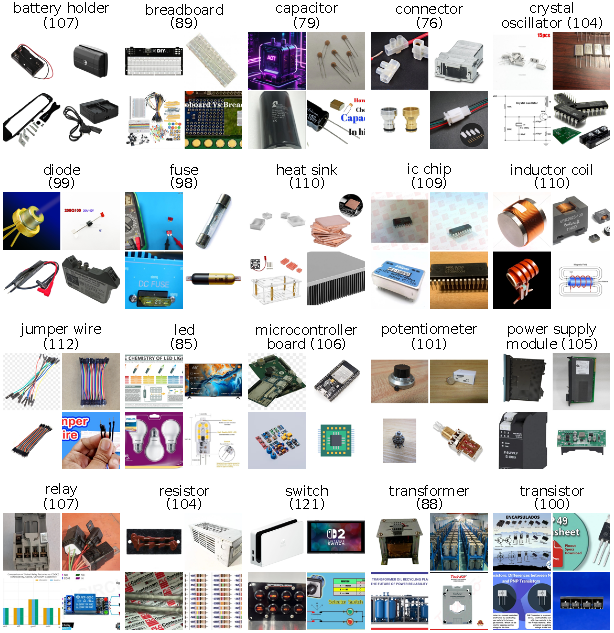
\includegraphics[width=0.82\textwidth]{fig02_examples_per_class.pdf}
\caption{Four random training images of every class (in brackets: training images of the class). The mix of product
photos, close-ups, renders, diagrams and off-topic pictures (e.g.\ the game console under \cls{switch}, the
infographic under \cls{led}) is typical of the dataset.}
\label{fig:examples}
\end{figure}

\subsection{Cleaning, label checking and corrections}\label{sec:cleaning}
The cleaning pipeline records a dataset manifest and an audit of all exclusions and duplicate groups;
\cref{tab:cleaning} summarises the counts.
\begin{enumerate}[leftmargin=*]
\item \textbf{Decoding.} Every file was decoded and stored as an RGB JPEG (the unique files were \nJPEG JPEG,
\nWEBP WebP, \nPNG PNG, \nAVIF AVIF, \nGIF GIF and \nMPO MPO files; \nAlpha transparent images were composited on
white). No file was corrupt.
\item \textbf{Exact duplicates.} Files with identical SHA-256 hashes were collapsed into one image (\nDupRedundant
redundant copies in \nDupGroups groups). \nConflictGroups groups (\nConflictFiles files) held the same image under two
class folders, e.g.\ \cls{fuse} and \cls{relay}; their labels contradict each other, so they were removed,
leaving \nRows images.
\item \textbf{Near-duplicates.} Re-encoded or resized copies were linked when their perceptual-hash distance (the
Hamming distance between pHash codes) was at most \phashRadius and the cosine similarity of their CLIP ViT-B/32
\citep{radford2021clip} embeddings at least \cosWithPhash, or when the cosine alone was at least \cosOnly. This gave \nNearDupClusters clusters with \nNearDupRows images (sizes 2 to \maxClusterSize), which are
kept but always assigned to the same split (\cref{sec:split}).
\item \textbf{Irrelevant or uncertain samples.} A CLIP zero-shot screen compares each image with the 20 class prompts
and \nDistractors distractor concepts (person, car, food, logo, text screenshot, cartoon or game art, circuit
schematic, website screenshot, collage) and flags it when the distractor probability mass exceeds \oodThreshold. It
flagged \nOOD images (\pctOOD\%), concentrated in classes whose names are common words: \nSwitchOOD of \nSwitch
\cls{switch} images (mostly Nintendo Switch consoles) and \nTransformerOOD of \nTransformer \cls{transformer} images
(toy robots, cartoons). Flagged images are kept and reported separately: in earlier 5-fold cross-validation,
dropping them from training lowered the accuracy of a linear classifier on frozen SigLIP features (a linear
probe, \cref{sec:modelC}) from \abKeepAcc to \abDropAcc overall and from \abKeepIn to \abDropIn on unflagged images.
\item \textbf{Label errors.} A confident-learning audit \citep{northcutt2021confident} on out-of-fold probe
probabilities listed \nLabelIssues images whose given label is improbable while another class is highly probable.
\end{enumerate}
\textbf{How labels were obtained, checked and corrected.} Labels come from the search query. They were checked
automatically (conflicting duplicates, CLIP screen, confident-learning audit) and by inspecting image review sheets. The only correction applied was the removal of the \nConflictGroups conflicting groups; we
did not relabel images, which would need a manual review of all \nRows images by more than one annotator. The test
labels therefore contain the same noise as the training labels, which caps every model's measurable accuracy.

\begin{table}[!tbp]
\centering\footnotesize
\caption{Cleaning pipeline; indented rows break down the row above.}
\label{tab:cleaning}
% generated by docs/itri626_report/make_tables.py -- do not edit by hand
\begin{tabular}{@{}lrl@{}}
\toprule
Step & Count & Action \\
\midrule
Raw image files in the Kaggle download & 3,530 & -- \\
Unique files (distinct SHA-256 of the bytes) & 2,943 & -- \\
\quad redundant exact copies (533 duplicate groups) & 587 & collapsed to one \\
\quad corrupt or undecodable files & 0 & -- \\
\quad duplicate groups with conflicting labels (27 files) & 13 & removed \\
Final images (rows of the manifest) & 2,930 & kept \\
\quad rows in near-duplicate clusters (91 clusters, size 2--29) & 234 & kept, grouped \\
\quad split units (clusters incl.\ singletons) & 2,787 & -- \\
\quad rows flagged out-of-scope by the CLIP screen & 816 & kept, flagged \\
\bottomrule
\end{tabular}

\end{table}

\subsection{Class imbalance}\label{sec:imbalance}
After cleaning, the largest class (\cls{\classMaxName}, \classMax images) is \imbalance times the smallest
(\cls{\classMinName}, \classMin); training classes have \trainMin--\trainMax images and test classes
\testMin--\testMax (\cref{tab:dataset}, \cref{fig:counts} in \cref{app:extra}). Because the imbalance is mild we used
no class weights and no re-sampling. Instead the split is stratified by class, early stopping and model
selection use validation macro-F1 (every class counts equally), and we report macro averages and weighted F1.

\subsection{Train/validation/test split and leakage prevention}\label{sec:split}
The unit of splitting is the duplicate cluster: a near-duplicate cluster or a single image without
near-duplicates (\nClusters clusters). We split in two stages and always keep a cluster whole. First,
StratifiedGroupKFold (scikit-learn \citep{pedregosa2011sklearn}; 7 folds, shuffled, seed
\splitSeed) partitions the clusters, and the fold whose class distribution is closest (total-variation distance) to
the overall one becomes the test set (\nTest images), which is held out (``sealed'') until the final
evaluation. Second, the remaining 2,512 development images are divided by the same method into five grouped folds:
fold~0 is the validation set (\nVal) and folds 1--4 form the training set (\nTrain), i.e.\
\pctTrain/\pctVal/\pctTest\%, close to the 70/15/15 split suggested in the brief.
The class distribution of each split is in \cref{tab:dataset}. The manifest fingerprint is \fingerprint.
The exported splits, notebook and report-generation checks verify that no image or duplicate cluster occurs in two splits.
Grouping matters: in the dataset's original random file split (counted over the raw file
entries), \legValCopies of \legValEntries
validation and \legTestCopies of \legTestEntries test entries are byte-identical copies of a training file, which
inflates scores \citep{barz2020cifair, kapoor2023leakage} (\cref{sec:further}). The test set was used once per model, after all choices had been fixed on validation data.

\subsection{Ethical, privacy and licensing considerations}\label{sec:ethics}
The task uses no health or personal records, and no person is a subject of the classification. As a web scrape,
the data contain incidental people (the CLIP screen names ``person'' as the top distractor for \nPersonTop images) and trademarks (game consoles, brand logos). We identify no one; such images appear in
our figures only as small thumbnails from the public dataset. Use follows \cref{sec:source}: the
source is acknowledged, the use is non-commercial and educational, and the images are not redistributed in the
repository (they are rebuilt from the Kaggle download, \cref{app:repro}). The 407 photographs of the supplementary web
holdout (\cref{sec:further}) are from Wikimedia Commons under public-domain or Creative-Commons licences; author,
licence and source of each are recorded in the accompanying attribution register. Pretrained weights come from
their official timm releases \citep{wightman2019timm}. The main risk is over-trust in a wrong label,
which is why we report confidence and a reject option. Web search results may also over-represent clean product
shots, so performance on cluttered workbench photographs can be lower (cf.\ the Wikimedia holdout in
\cref{sec:further}).

% ------------------------------------------------------------------------------------------------- 3
\section{Methodology, selected models and transfer learning}\label{sec:method}

\Cref{fig:workflow} shows the workflow. The same split files feed all four models; each is selected on the
validation set only and scored once on the test set.

\begin{figure}[!tbp]
\centering
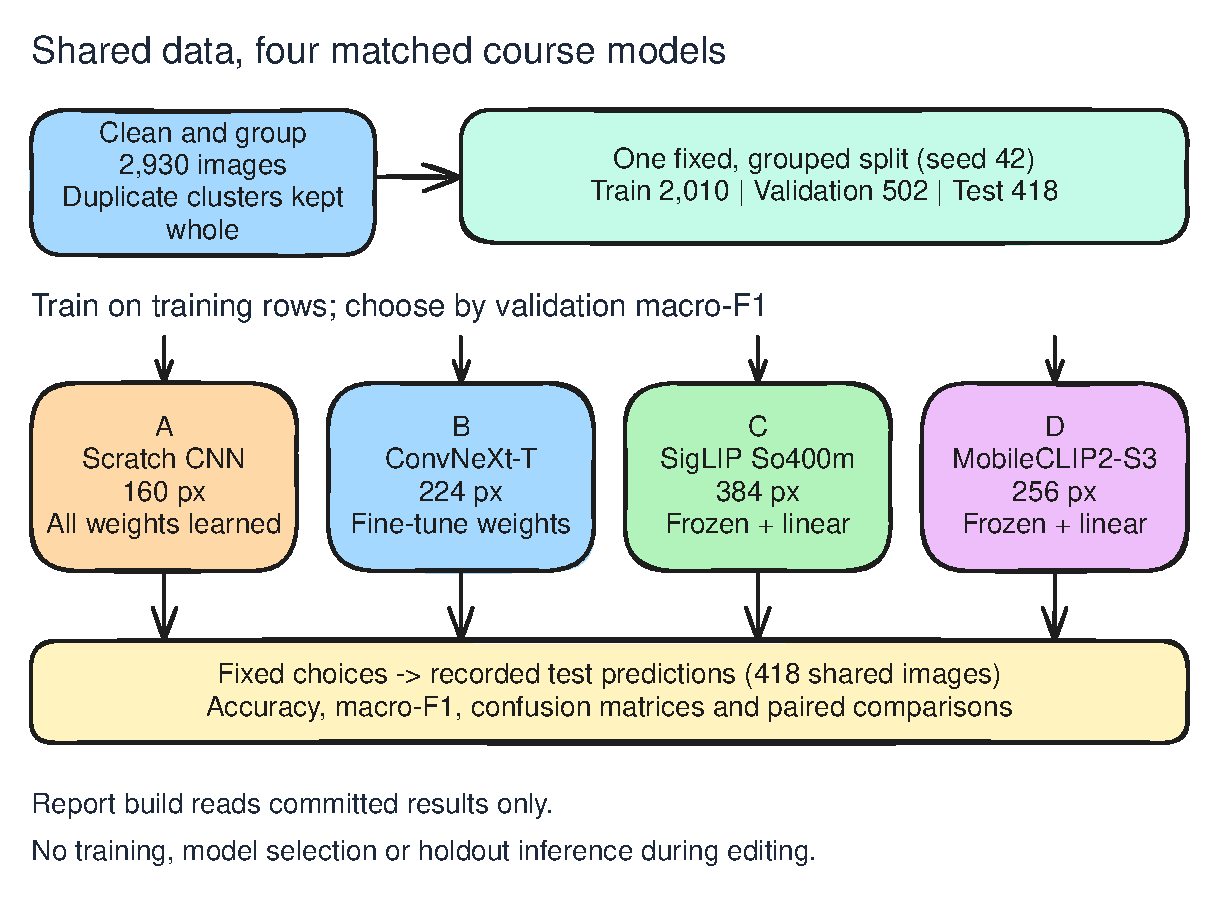
\includegraphics[width=\textwidth]{diagrams/workflow.pdf}
\caption{Shared preparation and evaluation of A--D. Duplicate clusters remain whole across the fixed split.
All choices precede test scoring. Editable Excalidraw sources and vector exports accompany the report.}
\label{fig:workflow}
\end{figure}

\Needspace{7\baselineskip}
\subsection{Model A: VGG-style CNN trained from scratch}
A VGG-style network \citep{simonyan2014vgg} written for this project:
a stride-2 stem convolution, four stages of two $3\times3$ convolution--BatchNorm \citep{ioffe2015bn}--ReLU blocks
(32, 64, 128, 256 channels) with max-pooling between stages, global average pooling, dropout 0.3 and a linear
classifier; \paramsA parameters with He initialisation \citep{he2015delving} and no pretrained weights. It
shows what can be learned from about 2,000 images alone.

\subsection{Model B: fine-tuned ConvNeXt-Tiny}
ConvNeXt \citep{liu2022convnext} modernises the ResNet design \citep{he2016resnet} with $7\times7$ depthwise
convolutions, inverted bottlenecks, LayerNorm and GELU. We use the Tiny variant (\paramsB parameters) with the
timm weights, pretrained on ImageNet-22k and fine-tuned on
ImageNet-1k \citep{russakovsky2015imagenet}. The 1000-class head is replaced by a new 20-class linear layer, which is
trained alone in the first epoch so that its large initial gradients do not disturb the pretrained features
\citep{kumar2022finetuning}. Afterwards all layers are trained, with layer-wise learning-rate decay 0.8 so that early,
generic layers change less than late, task-specific ones. Fine-tuning ImageNet networks is the standard transfer
recipe for small datasets \citep{yosinski2014transferable, kornblith2019transfer}.

\subsection{Model C: frozen SigLIP So400m ViT with a linear head}\label{sec:modelC}
The Vision Transformer \citep{dosovitskiy2020vit} splits an image into patches and processes the patch tokens with
self-attention. SigLIP \citep{zhai2023siglip} trains a ViT image encoder and a text encoder on WebLI (a web-scale
image--text collection) with a pairwise sigmoid loss. We use its shape-optimised So400m/14 encoder at $384\times384$ pixels (27 blocks,
width 1152, patch size 14; timm weights pretrained on WebLI). The backbone
is frozen. Each image is encoded once into its attention-pooled 1152-dimensional embedding; the features are
standardised with the training-split mean and standard deviation, and only one linear layer with 1,152 inputs and 20 outputs
(\paramsHead parameters) with softmax output is trained with cross-entropy and AdamW, i.e.\ the linear-probe
protocol used for image--text models \citep{radford2021clip}.

\subsection{Model D: frozen MobileCLIP2-S3 hybrid with a linear head}\label{sec:modelD}
MobileCLIP2 \citep{faghri2025mobileclip2} provides compact image--text encoders. Its S3 image encoder is a
FastViT convolution--attention hybrid \citep{vasu2023fastvit}, at $256\times256$ pixels with 122,775,668 parameters
(3.5 times fewer than C; weights pretrained on DFNDR-2B). D uses C's frozen-feature procedure,
training-only standardisation and selection rule, with a linear head with 3,072 inputs and 20 outputs (61,460 trainable parameters).
It was selected using development folds to study the accuracy--cost trade-off.
A--C meet the brief's three named families; D is supplementary, with approval as an additional family still unconfirmed.

\subsection{Rationale for the models and evaluation protocol}
The brief lists a small custom CNN, ConvNeXt and the Vision Transformer as separate suitable families; our models
take one from each (plain CNN, modernised CNN, Vision Transformer) and span the transfer-learning
spectrum: no transfer (A), full fine-tuning of supervised ImageNet features (B) and frozen features from web-scale
image--text pretraining (C and D). Between B and C, architecture and pretraining data change together, so the comparison
measures model plus pretraining as available to a practitioner; the supplementary benchmark
(\cref{sec:further}) provides additional comparisons, without isolating a causal effect of architecture.

\textbf{Evaluation.} On the test set we compute per-class precision, recall and F1, their macro averages (all classes equal) and weighted
averages (by support), accuracy, balanced accuracy (equal to macro recall) and log-loss. Uncertainty is estimated with
2,000 bootstrap resamples of the test images \citep{efron1979bootstrap}; pairs of models are compared on the same
images with a paired bootstrap of the accuracy difference and an exact McNemar test \citep{mcnemar1947}, which
tests whether, on the images where exactly one of the two models is right, each model is right equally often.

% ------------------------------------------------------------------------------------------------- 4
\section{Experimental setup and hyperparameters}\label{sec:setup}

\subsection{Preprocessing}
Every image is decoded to 8-bit RGB, and each model uses the input size and normalisation of its weights. For evaluation (validation, test, and the
feature extraction of C and D) the short side is resized to the input size divided by the crop fraction (0.875 for A
and B, 0.9 for C, 1.0 for D) and the centre square is cut out:
183$\to$160\,px bilinear for A, 256$\to$224\,px bicubic for B, 427$\to$384\,px bicubic for C; 256\,px bicubic, with no short-side border removed, for D. Pixels are scaled to
$[0,1]$ and normalised per channel (mean and standard deviation 0.5 for A and C; ImageNet statistics for B; CLIP statistics for D, recorded in its run JSON).

\subsection{Augmentation (training data only)}
A and B are trained with RandomResizedCrop (aspect ratio 0.75--1.33), horizontal flips ($p=0.5$) and
RandAugment with two operations of magnitude 9 \citep{cubuk2020randaugment}; A also uses colour jitter 0.2 and a
wider crop range (scale 0.35--1 instead of 0.5--1), because a network trained from scratch needs stronger
regularisation (\cref{fig:aug}). Validation and test images always receive the deterministic evaluation transform.
The transformations are realistic for this domain: web photos of parts are taken at arbitrary zoom and framing
(random crops), components have no canonical left--right orientation (horizontal flips), and lighting, white balance
and compression vary between shops and phones (RandAugment's photometric operations, colour jitter). Vertical flips
were not used because printed text and lighting in product shots have a natural ``up'', and MixUp/CutMix were not used
because blended components cannot occur. C and D use no augmentation: their features are computed once from the evaluation
crop, which keeps the frozen-feature protocol simple and cheap.

\begin{figure}[!tbp]
\centering
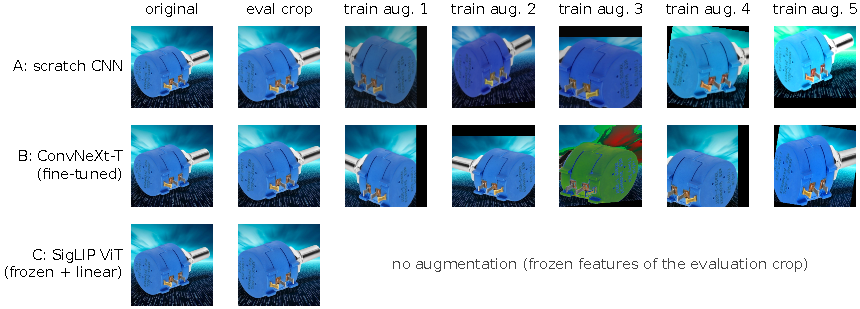
\includegraphics[width=\textwidth]{fig03_augmentation.pdf}
\caption{One training image, its evaluation crop and five random training augmentations per model. C uses frozen
features of the evaluation crop; D (not pictured) likewise uses a deterministic 256 px view without augmentation.}
\label{fig:aug}
\end{figure}

\subsection{Hyperparameters}
\Cref{tab:hparams} lists every training setting in two parts. Settings differ where the architectures require it. A randomly
initialised CNN needs a high learning rate, many epochs and strong augmentation. A pretrained network needs a small
learning rate and few epochs. A linear head on frozen, standardised features needs neither augmentation nor a
learning-rate schedule. The recipe of B was fixed earlier in the project's grouped 5-fold cross-validation
benchmark on the 2,512 development images only, and so was A's apart from its
schedule: the benchmark's 120-epoch budget stopped A before it had converged, and the improvement study of
\cref{sec:improveA}, again on the development folds only, lengthened it to \maxEpochsA epochs (patience 40). The
\nTest test images were never used for any of this. For each frozen head, the weight decay is selected on the validation set from
$\{10^{-4},10^{-3},10^{-2},10^{-1}\}$ (\cref{tab:wdgrid}, \cref{app:extra}). The \nTies smallest values
($10^{-4}$ to $10^{-2}$) reached the identical best validation macro-F1, because AdamW's decoupled decay \citep{loshchilov2019adamw} is negligible over a
few dozen epochs at this learning rate; the tie was broken by the rule, fixed before the grid was run, that the
smallest value wins. A and B use label smoothing 0.1 \citep{szegedy2016inception} and a cosine schedule
\citep{loshchilov2017sgdr}. All models are early-stopped on validation macro-F1, and the best validation epoch is
tested. D uses the same grid and tie-break; all four values tied (\cref{tab:wdgridD}).



\subsection{Software, hardware and reproducibility}\label{sec:software}
The models are implemented in PyTorch \citep{paszke2019pytorch} with timm \citep{wightman2019timm};
scikit-learn \citep{pedregosa2011sklearn} provides the split and the reference probe, and uv \citep{astral2024uv}
pins the environment. B was trained on one \gpuName with \gpuMem\,GiB of memory (all versions and the hardware are in
\cref{tab:env}, \cref{app:extra}). The final run of A was trained after the improvement study (\cref{sec:improveA})
on a second machine, one \gpuNameA with \gpuMemA\,GiB (Windows 11; the same code, lock file and seed; its software
versions are recorded with the run metadata). Peak GPU memory was
\vramA\,MB for A and \vramB\,MB for B, and the heads of C and D were trained on the CPU from cached features. D's feature extraction and timing used the second machine (RTX 4070 Laptop). The training seed is 0
and the split seed \splitSeed. GPU training of A is not bit-for-bit reproducible (non-deterministic cuDNN kernels), so
a re-run can differ slightly. Result files, the executed comparison notebook and reproduction instructions are available in the project repository
(\cref{app:repro}).

\textbf{Fairness.}\label{sec:fairness} All four models use the same \nTrain training, \nVal validation and \nTest
test images, the same selection rule (best validation macro-F1) and a single test evaluation each, with no test-time
augmentation. Tuning effort is comparable: the recipes of A and B come from the earlier development-set benchmark,
and each frozen head's only tuned setting is a four-value weight-decay grid on the validation set (\cref{tab:wdgrid}). Budgets
differ only where the architecture requires it (\cref{tab:hparams}): A receives \maxEpochsA epochs and converges within
them (best epoch \bestA), whereas B begins to overfit within \maxEpochsB. B and C also differ in pretraining data, which we treat as
part of each method (\cref{sec:limits}). D's crop fraction 1.0 was fixed on development data; C retains 0.9. No test number led to a change of any setting.


% ------------------------------------------------------------------------------------------------- 5
\section{Results and model comparison}\label{sec:results}

\subsection{Overall test performance}
\Cref{tab:test} gives the test metrics: C (accuracy \accC, macro-F1 \foneC) $>$ D (\accD, \foneD)
$>$ B (\accB, \foneB) $>$ A (\accA, \foneA). Individual 95\% bootstrap intervals overlap for C and D;
the paired comparison favours C (39 images only C gets right, 18 only D; $p=$\pvalCD).
All six pairwise McNemar tests reject equal accuracy (\cref{tab:pairwise}; unadjusted $p$-values).
Balanced accuracy and macro and weighted averages are close because the classes are nearly balanced.
Test accuracy is within about two points of validation accuracy at the selected epoch for all four models
(\cref{tab:curves}). C has the lowest log-loss (\loglossC); this favours its probabilistic predictions on average,
although log-loss alone does not establish calibration.

The reference rows use different fitting procedures and are not matched main models. R1 fits a scikit-learn
logistic-regression head on C's training features (\accRA). R2 (Deployed) refits on train plus validation and fuses
with SigLIP's zero-shot head (\accRB); R3 (Small) does the same with MobileCLIP2-S3 (\accRC).
Their extra fitting data and heads prevent attributing these gains solely to backbone choice (\cref{fig:protocols}).

\begin{table}[!tbp]
\centering\footnotesize
\caption{Test-set metrics ($n=\nTest$, same images for all models). Bold:
best main model. CI: 95\% percentile bootstrap (2,000 resamples).}
\label{tab:test}
\setlength{\tabcolsep}{2pt}
% generated by docs/itri626_report/make_tables.py -- do not edit by hand
\begin{tabular}{@{}lccccccc@{}}
\toprule
Model & Acc. & Bal.\ acc. & Macro P & Macro R & Macro F1 & Weighted F1 & Log loss \\
\midrule
A: custom CNN & 0.354 & 0.343 & 0.339 & 0.343 & 0.336 & 0.347 & 2.334 \\
\quad 95\% CI & 0.306--0.400 & & & & 0.288--0.372 & & \\
B: ConvNeXt-T FT & 0.636 & 0.630 & 0.642 & 0.630 & 0.628 & 0.632 & 1.346 \\
\quad 95\% CI & 0.591--0.682 & & & & 0.578--0.668 & & \\
C: SigLIP ViT + linear & \textbf{0.823} & \textbf{0.821} & \textbf{0.827} & \textbf{0.821} & \textbf{0.817} & \textbf{0.820} & \textbf{0.614} \\
\quad 95\% CI & 0.787--0.859 & & & & 0.774--0.851 & & \\
\midrule
\multicolumn{8}{@{}l}{\textit{Reference rows (same frozen SigLIP features as C; not additional models)}} \\
R1: SigLIP + sklearn probe & 0.833 & 0.830 & 0.838 & 0.830 & 0.829 & 0.832 & 0.606 \\
R2: deployed fused model & 0.837 & 0.836 & 0.843 & 0.836 & 0.834 & 0.836 & 0.527 \\
\bottomrule
\end{tabular}

\end{table}

\begin{table}[!tbp]
\centering\footnotesize
\caption{Paired comparisons on the same \nTest test images: accuracy difference $\Delta$ as a proportion
($\times100$ = percentage points, as in the text), paired-bootstrap interval, discordant counts, exact McNemar test.}
\label{tab:pairwise}
% generated by docs/itri626_report/make_tables.py -- do not edit by hand
\begin{tabular}{@{}lrcrrr@{}}
\toprule
Pair & $\Delta$ accuracy & 95\% CI & Only 1st right & Only 2nd right & McNemar $p$ \\
\midrule
B $-$ A & +0.237 & +0.189 to +0.289 & 119 & 20 & $2.4\times10^{-18}$ \\
C $-$ B & +0.187 & +0.141 to +0.232 & 92 & 14 & $3.1\times10^{-15}$ \\
C $-$ A & +0.423 & +0.373 to +0.474 & 184 & 7 & $1.1\times10^{-45}$ \\
\bottomrule
\end{tabular}

\end{table}

\subsection{Learning curves}
\Cref{fig:curves} shows training and validation loss and validation accuracy and macro-F1 per epoch;
\cref{tab:curves} (\cref{app:extra}) gives the values at the selected epoch. Losses are plain cross-entropy.
\begin{itemize}[leftmargin=*]
\item A improves slowly for most of its \maxEpochsA-epoch budget and is selected at epoch \bestA. There its
training accuracy is \trainAccA but its validation accuracy only \valAccA. The validation loss is lowest at epoch
\minValCEepA (\minValCEA; chance level $\ln 20=\lnTwenty$) and then rises to \valCEA while validation accuracy and
macro-F1 still improve: the network grows more confident without changing many decisions, and in its second
hundred epochs it also fits the training set (training cross-entropy \trainCEA). The 120-epoch schedule of the
earlier benchmark stopped it before this point (\cref{sec:improveA}).
\item B profits from its pretrained features at once: validation accuracy passes 0.5 in epoch \epHalfB and
plateaus near \valAccB, while training accuracy rises to \finalTrainAccB and validation loss stays at about \valCEB,
i.e.\ a 28-million-parameter network overfits a small, noisy training set. The cosine schedule and early stopping
(best epoch \bestB of \epochsB) keep it from getting worse.
\item C passes 0.75 validation accuracy in epoch \epTqC and reaches \valAccC. Training accuracy goes to
\finalTrainAccC, since 1,152 standardised features are almost linearly separable for 2,010 images. Validation loss is
lowest in epoch \minValCEepC (\minValCEC) and then creeps up while accuracy and macro-F1 stay flat: the head grows more
confident without changing many decisions. Early stopping selected epoch \bestC.
\item D reaches validation accuracy \valAccD{} and macro-F1 \valFoneD{} at epoch 11 of 31; its 3,072-dimensional features support the same inexpensive head-fitting procedure.
\end{itemize}

\begin{figure}[!tbp]
\centering
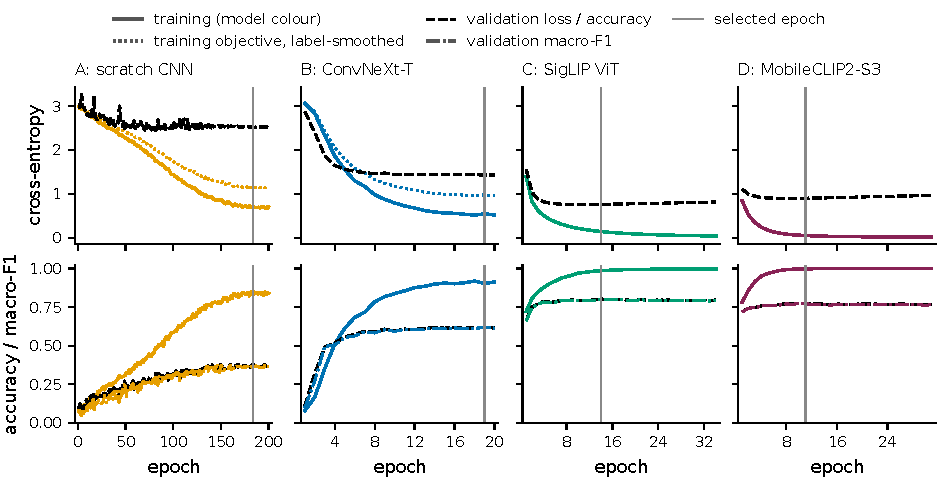
\includegraphics[width=\textwidth]{../../results/itri626/figures_four_models/fig04_learning_curves.pdf}
\caption{Learning curves (one column per model). Top: cross-entropy; dotted: label-smoothed training objective
(A, B). Bottom: training accuracy, validation accuracy and macro-F1. Training curves of A and B are measured on
augmented batches; the grey line marks the epoch whose weights were tested.}
\label{fig:curves}
\end{figure}


\subsection{Per-class results and confusion matrices}
\Cref{fig:perclass} plots the per-class test F1; the full per-class precision, recall and F1 values are in
\cref{tab:perclass,tab:perclassD} (\cref{app:perclass}). \MC is strongest overall; its weakest class is
\cls{\worstC} (F1 \worstFoneC, recall \recResC) and its strongest \cls{\bestClsC} (\bestFoneC). B is weakest on
\cls{\worstB} (F1 \worstFoneB, recall \recFuseB). A exceeds F1 0.5 only for a few visually distinctive classes
(\cls{microcontroller board}, \cls{switch}, \cls{jumper wire}, \cls{heat sink}). D is weakest on \cls{led} (F1 0.61) and strongest on \cls{potentiometer} (0.93). The confusion matrices
(\cref{fig:cm}) show A's errors spread over the whole matrix, B's concentrated in a few blocks, and those of C and D almost
diagonal; \cref{sec:errors} analyses the largest off-diagonal entries.

\begin{figure}[!tbp]
\centering
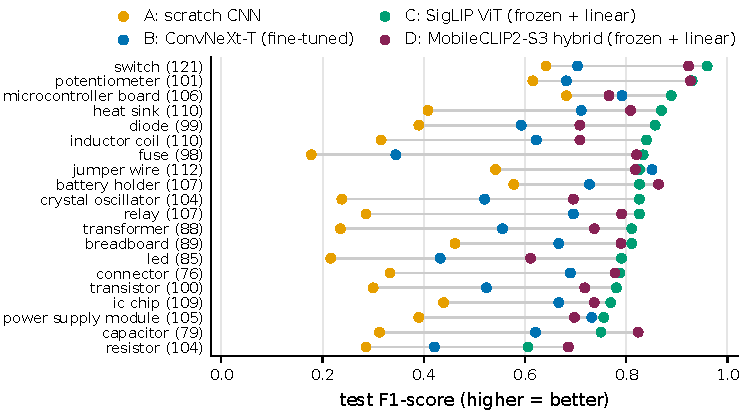
\includegraphics[width=0.9\textwidth]{../../results/itri626/figures_four_models/fig07_per_class_f1.pdf}
\caption{Per-class test F1 of the four models, sorted by \mC; the number after each class is its training-set
size.}
\label{fig:perclass}

\end{figure}

\subsection{Correct and incorrect predictions}
\Cref{fig:galleries} shows C's six random correct predictions and its six most confident errors with
true class, prediction and softmax confidence. A and B appear in \cref{fig:galleryAB}, and D in \cref{fig:galleryD}. Many of C's confident errors are images that do not show the labelled component: a DIP chip
labelled \cls{transistor}, a breadboard power module labelled \cls{breadboard}, a fibre-optic pigtail and a coaxial
plug labelled \cls{jumper wire}, and an icon sheet and a ``Capacitor vs Resistor'' banner labelled \cls{resistor}. A's most
confident errors include a sheet of package drawings labelled \cls{diode}, an LED arrow sign labelled \cls{power supply
module} and handwritten notes labelled \cls{inductor coil}.

\begin{figure}[!tbp]
\centering
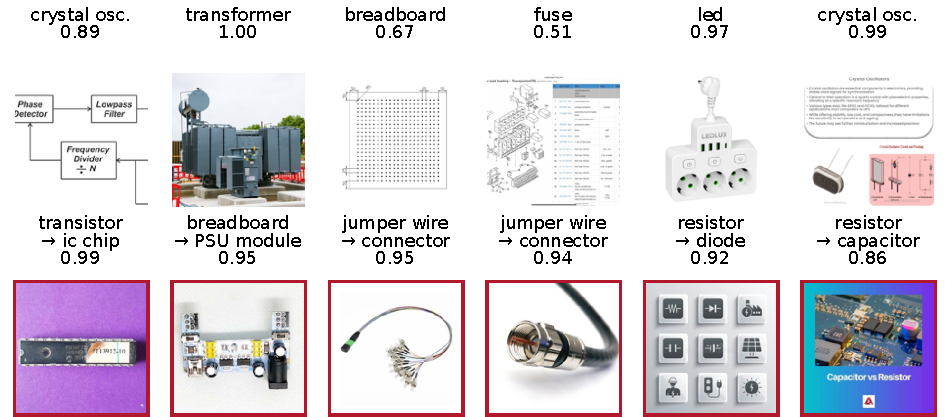
\includegraphics[width=\textwidth]{figures/gallery_C_siglip_so400m_linear.pdf}
\caption{Model C: six random correct predictions (top row) and six most confident errors (bottom row, red frame,
true $\to$ predicted). Confidence is the softmax probability of the predicted class.
MCU board = microcontroller board; PSU module = power supply module; crystal osc.\ = crystal oscillator;
batt.\ holder = battery holder. A and B are shown in \cref{fig:galleryAB}; D in \cref{fig:galleryD}.}
\label{fig:galleries}
\end{figure}

\subsection{Agreement between the models and computational cost}
A, B and C are right on \allRight test images and all three wrong on \allWrong (\cref{fig:agree}). \onlyC
images are recognised only by C and \bcNotA by B and C but not A, whereas C is wrong on only \cWrongOther images that A
or B get right (examples in \cref{fig:disagree}). D recognises 14 of the \allWrong images that A, B and C all miss, leaving 43 that no model gets right, and is wrong on 27 images that A or B get right.

\begin{figure}[!tbp]
\centering
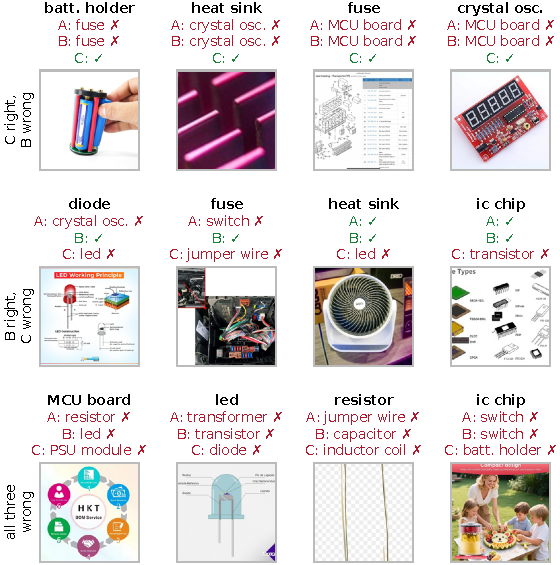
\includegraphics[width=\textwidth]{fig10_disagreements.pdf}
\caption{Disagreements among A--C. Rows: C right and B wrong; B right and C wrong; all three wrong.
Titles give the true class (bold) and each model's prediction; ticks mark correct predictions and crosses errors.
Abbreviations as in \cref{fig:galleries}. The agreement counts are plotted in \cref{fig:agree}.}
\label{fig:disagree}
\end{figure}

Accuracy has a price (\cref{tab:eff} in \cref{app:extra}): C needs \gpuMsC\,ms per
image on the GPU at batch size 1, about \gpuRatioCB times as long as B (\gpuMsB\,ms), and \cpuMsC\,ms on an 8-thread
CPU, about \cpuRatioCB times as long as B (\cpuMsB\,ms); its frozen backbone weighs \fpMBC\,MB in fp32.
D uses \fpMBD\,MB of fp32 weights. On D's PC, its 15.16 ms GPU and 111.5 ms CPU times compare with
37.94 and 1,563.3 ms for C's tower: about 2.5 and 14 times faster, respectively. This is a same-machine
anchor, not a ratio against C's different-PC table row; it also excludes C's head and preprocessing.




% ------------------------------------------------------------------------------------------------- 6
\section{Discussion, limitations and error analysis}\label{sec:discussion}

\subsection{Why the models differ}\label{sec:why}
The ranking follows how much relevant visual knowledge each model brings to a 2,010-image problem, rather than
depth or parameter count. A starts from random weights and must learn edges, textures, shapes and classes at
once from about 100 images per class; its learning curves show it is data-limited, as does the improvement study of
\cref{sec:improveA} (more epochs helped; more capacity, residual blocks, stronger augmentation and better
initialisation did not), and its per-class F1 correlates with the number of training images (Spearman $\rho$ over
the 20 classes \rhoA, against \rhoB for B, \rhoC for C and +0.20 for D). B re-uses ImageNet-22k features that already encode objects, materials and shapes, so it learns quickly;
but ImageNet contains few electronic parts, so the features are generic, and fine-tuning all 28 million parameters on
2,010 noisy images shows a generalisation gap (training accuracy \finalTrainAccB against \valAccB on validation). C uses a
428-million-parameter encoder pretrained on web image--text pairs. Its embedding already separates the classes:
SigLIP zero-shot classification, with no training at all, reaches macro-F1 \bmZeroSiglip in the benchmark
(\cref{sec:further}). It is also the least affected by off-topic images (\accOODC on flagged test images against
\accOODB for B, \cref{sec:errors}), plausibly because such images resemble its web pretraining data. Freezing the
backbone means label noise cannot distort it, and
training the \paramsHead head parameters takes \timeC\,s for the whole grid on cached features.
D repeats this strategy with a smaller hybrid: \diffCD{} accuracy points below C and \diffDB{} above B.
These results support the value of the representation; architecture and pretraining are not independently controlled.

\subsection{Error analysis}\label{sec:errors}
\textbf{Look-alike components.} \Cref{tab:confused} lists the most frequent confusions. C's largest are
\cls{resistor} $\to$ \cls{inductor coil} (\cmResIndC) and \cls{jumper wire} $\to$ \cls{connector} (\cmJumpConC); B's are
\cls{resistor} $\to$ \cls{crystal oscillator} (\cmResXtalB) and \cls{ic chip} $\to$ \cls{microcontroller board}
(\cmIcMcuB). These pairs share shapes: colour-banded axial bodies (some inductors look like fat resistors), cables
with plugs, chips mounted on boards. \cls{Resistor} is C's hardest class: precision \precResC but recall only
\recResC, partly because several test ``resistors'' are icon sheets, banners or schematics. A's confusions (e.g.\
\cls{fuse} $\to$ \cls{connector}, \cls{fuse} $\to$ \cls{switch}) are spread widely and often have no obvious visual
explanation, consistent with a model that has not learned robust shape features. \cls{Diode} and \cls{led} are
related devices that are often shown together in infographics (\cmDiodeLedC of C's errors are \cls{diode} $\to$ \cls{led}).
D's largest is \cls{ic chip} $\rightarrow$ \cls{microcontroller board} (4), which it shares with B, and it shares \cls{jumper wire} $\rightarrow$ \cls{connector} (3) with C. Summed over all four models, the most frequent confusions are \cls{jumper wire} $\rightarrow$ \cls{connector} (10), \cls{transistor} $\rightarrow$ \cls{diode} (10) and \cls{resistor} $\rightarrow$ \cls{crystal oscillator} (9).

\begin{table}[!tbp]
\centering\scriptsize
\caption{Most frequent test confusions (true $\rightarrow$ predicted) per model, from their recorded confusion matrices; equal counts are listed alphabetically. MCU board: microcontroller board; crystal osc.: crystal oscillator; PSU module: power supply module.}
\label{tab:confused}
\setlength{\tabcolsep}{3.5pt}
% four-model version of generated/tab_confused.tex, from results/itri626/metrics.json (hand-over, see D_ANALYSIS_INSERTS.md)
\begin{tabular}{@{}clrVlrVlrVlr@{}}
\toprule
 & \multicolumn{2}{c}{\msq{A}A} & \multicolumn{2}{c}{\msq{B}B} & \multicolumn{2}{c}{\msq{C}C} & \multicolumn{2}{c}{\msq{D}D} \\
\cmidrule(lr){2-3} \cmidrule(lr){4-5} \cmidrule(lr){6-7} \cmidrule(lr){8-9}
\# & True $\rightarrow$ predicted & $n$ & True $\rightarrow$ predicted & $n$ & True $\rightarrow$ predicted & $n$ & True $\rightarrow$ predicted & $n$ \\
\midrule
1 & crystal osc. $\rightarrow$ relay & 5 & resistor $\rightarrow$ crystal osc. & 5 & resistor $\rightarrow$ inductor coil & 4 & ic chip $\rightarrow$ MCU board & 4 \\
2 & inductor coil $\rightarrow$ resistor & 4 & ic chip $\rightarrow$ MCU board & 4 & jumper wire $\rightarrow$ connector & 3 & inductor coil $\rightarrow$ transformer & 3 \\
3 & transistor $\rightarrow$ diode & 4 & capacitor $\rightarrow$ diode & 3 & battery holder $\rightarrow$ led & 2 & jumper wire $\rightarrow$ connector & 3 \\
4 & battery holder $\rightarrow$ heat sink & 3 & heat sink $\rightarrow$ crystal osc. & 3 & breadboard $\rightarrow$ PSU module & 2 & led $\rightarrow$ diode & 3 \\
5 & capacitor $\rightarrow$ relay & 3 & led $\rightarrow$ switch & 3 & capacitor $\rightarrow$ inductor coil & 2 & MCU board $\rightarrow$ crystal osc. & 3 \\
6 & connector $\rightarrow$ potentiometer & 3 & led $\rightarrow$ transistor & 3 & diode $\rightarrow$ led & 2 & relay $\rightarrow$ PSU module & 3 \\
\bottomrule
\end{tabular}

\end{table}

\textbf{Data quality matters more than class imbalance.} On the \nTestClean test images that the CLIP screen did not
flag, accuracy is \accCleanA (A), \accCleanB (B) and \accCleanC (C); on the \oodTest flagged ones it is \accOODA,
\accOODB and \accOODC. D scores \accCleanD{} on unflagged and \accOODD{} on flagged images. B loses most (\oodDropB points; A \oodDropA,
C \oodDropC, D \oodDropD), and C stays far ahead on flagged images, plausibly because its pretraining has seen such web content. A, B and C
fail on \allWrong test images, many of them infographics, diagrams or scenes without the labelled component, where
the label rather than the prediction is often questionable (\cref{fig:disagree}). Class imbalance, by contrast, is not
an important factor: the size ratio is only \imbalance, and C's per-class F1 is not significantly related to class
size ($\rho=\rhoC$, $p=\rhopC$).


\textbf{Confidence is informative.} C's mean softmax confidence is \confOkC on correct and \confBadC on wrong
predictions (B: \confOkB and \confBadB; D: 0.90 and 0.56), so a reject option can catch many errors \citep{chow1970reject,
geifman2017selective}. The deployed model uses one: at a confidence threshold of \ftThr it answers \ftCov\% of the
test images and is right on \ftAccepted of those.

\subsection{Can the scratch CNN be improved?}\label{sec:improveA}
A 19-experiment study used development folds only to test whether recipe changes close the gap
as documented in the supplementary scratch-CNN study. Resolution, capacity, depth, residual blocks,
regularisation, augmentation and initialisation changes produced no consistent gain. Training to convergence
(200 rather than 120 epochs) did help: five-fold macro-F1 rose by \imprSchedGain{} points, with gains on all folds
(\cref{tab:improveA}, \cref{app:benchmark}). That schedule is A in this report; its recorded test gain is
\imprTestGain{} macro-F1 points, not a selection criterion. It still overfits (\trainAccA{} training accuracy versus
\valAccA{} validation). On the independent Wikimedia set A reaches \imprHoldA{} macro-F1, against \whFone{} for
Deployed. The tested recipe improvements did not close the transfer-learning gap.

\subsection{Supporting evidence from the wider study}\label{sec:further}
The project's broader study (details in \cref{app:benchmark}) supports the comparison.
Grouped 5-fold cross-validation over eleven families reproduces the ordering (macro-F1: scratch CNN \bmScratch
with the benchmark's 120-epoch schedule, \imprFiveA with the 200-epoch schedule of \cref{sec:improveA};
ConvNeXt-T fine-tuned \bmConvnext, frozen SigLIP So400m probe \bmProbeSiglip), and every ImageNet-pretrained fine-tune
(\bmImagenetLo--\bmImagenetHi) stays below SigLIP zero-shot classification without any training (\bmZeroSiglip).
The dataset's original file-level split leaks duplicates and inflates linear-probe accuracy by \inflSiglip to
\inflResnet points, more for weaker models. On \whN fresh Wikimedia Commons photographs the deployed SigLIP-based model
(R2) scored \whAcc accuracy, close to its in-distribution result.

\subsection{Limitations}\label{sec:limits}
This comparison uses one training seed and one fixed test split, with about 21 images per class.
Unreviewed search-term labels, residual duplicates and CLIP-derived off-topic flags limit interpretation;
the screen shares a lineage with the frozen image--text encoders. Architecture, pretraining data and training
budgets change together, so the scores compare practical recipes rather than isolate their causes.
D also differs in evaluation crop and timing hardware; its weights have research-use restrictions.
C's cost (\paramsMC{} million parameters; \cpuMsC\,ms per CPU image) limits deployment.
The detailed limitations and provenance are retained in \cref{app:benchmark}; neither holdout should be reused for selection.


% ------------------------------------------------------------------------------------------------- 7
\section{Conclusion}\label{sec:conclusion}
On the fixed, duplicate-aware split, C (SigLIP, accuracy \accC, macro-F1 \foneC) leads D
(MobileCLIP2-S3, \accD, \foneD), B (ConvNeXt-T, \accB, \foneB) and A (scratch CNN, \accA, \foneA).
Both frozen encoders outperform the tested fine-tuned and scratch networks, although architecture and pretraining
remain confounded. Training A to convergence helped without closing the gap.

\textbf{Recommendation.} Choose C for accuracy when its memory and latency are acceptable. D trades
\diffCD{} accuracy points for 3.5 times fewer parameters and lower measured latency, subject to research-use
restrictions. B offers still lower latency. Deployed (R2, \accRB) and Small (R3, \accRC) refit on development
rows and fuse with zero-shot heads; they are distinct from C and D. Fast retains SigLIP at 308 px with INT8
TensorRT. Their fitting and timing protocols differ.

\textbf{Lessons learned.} On this small, noisy dataset, pretrained representation and a duplicate-aware split
matter more than the classifier fitted on top. Better labels and cleaner homonym classes are promising next steps;
future selection requires fresh evaluation data rather than further use of the spent holdouts.

\FloatBarrier
% ------------------------------------------------------------------------------------------------- 8
\renewcommand{\bibfont}{\small}\setlength{\bibsep}{2pt plus 1pt}
\bibliographystyle{ieeetr}
\bibliography{refs,extra}

% ------------------------------------------------------------------------------------------------- appendices
\clearpage
\appendix
\crefalias{section}{appendix}
\counterwithin{figure}{section}\counterwithin{table}{section}
\section{Detailed evaluation results}\label{app:perclass}
\Cref{tab:perclass} gives the per-class test precision, recall and F1 of A--C, and
\cref{tab:perclassrefs} those of R1 and R2 on the same test images. \Cref{tab:perclassD} adds D and R3 (Small). The per-class image counts of every
split are in \cref{tab:dataset}.

\begin{table}[htbp]
\centering\small
\caption{Per-class test precision (P), recall (R) and F1 ($n$ = test images per class). Best F1 among A--C per class in bold.}
\label{tab:perclass}
\setlength{\tabcolsep}{4pt}
% generated by docs/itri626_report/make_tables.py -- do not edit by hand
\begin{tabular}{@{}lrccccccccc@{}}
\toprule
 & & \multicolumn{3}{c}{\msq{A}A: scratch CNN} & \multicolumn{3}{c}{\msq{B}B: ConvNeXt-T} & \multicolumn{3}{c}{\msq{C}C: SigLIP ViT} \\
\cmidrule(lr){3-5} \cmidrule(lr){6-8} \cmidrule(lr){9-11}
Class & $n$ & P & R & F1 & P & R & F1 & P & R & F1 \\
\midrule
battery holder & 22 & 0.38 & 0.50 & 0.43 & 0.73 & 0.73 & 0.73 & 0.79 & 0.86 & \textbf{0.83} \\
breadboard & 19 & 0.53 & 0.47 & 0.50 & 0.65 & 0.68 & 0.67 & 0.83 & 0.79 & \textbf{0.81} \\
capacitor & 17 & 0.12 & 0.12 & 0.12 & 0.75 & 0.53 & 0.62 & 0.80 & 0.71 & \textbf{0.75} \\
connector & 16 & 0.18 & 0.19 & 0.18 & 0.77 & 0.62 & 0.69 & 0.76 & 0.81 & \textbf{0.79} \\
crystal oscillator & 21 & 0.29 & 0.33 & 0.31 & 0.45 & 0.62 & 0.52 & 0.76 & 0.90 & \textbf{0.83} \\
diode & 21 & 0.25 & 0.14 & 0.18 & 0.48 & 0.76 & 0.59 & 0.86 & 0.86 & \textbf{0.86} \\
fuse & 20 & 0.12 & 0.10 & 0.11 & 0.56 & 0.25 & 0.34 & 0.94 & 0.75 & \textbf{0.83} \\
heat sink & 23 & 0.67 & 0.43 & 0.53 & 0.73 & 0.70 & 0.71 & 0.87 & 0.87 & \textbf{0.87} \\
ic chip & 22 & 0.46 & 0.50 & 0.48 & 0.76 & 0.59 & 0.67 & 0.88 & 0.68 & \textbf{0.77} \\
inductor coil & 23 & 0.45 & 0.43 & 0.44 & 0.64 & 0.61 & 0.62 & 0.78 & 0.91 & \textbf{0.84} \\
jumper wire & 23 & 0.55 & 0.52 & 0.53 & 0.83 & 0.87 & \textbf{0.85} & 0.83 & 0.83 & 0.83 \\
led & 18 & 0.23 & 0.28 & 0.25 & 0.42 & 0.44 & 0.43 & 0.68 & 0.94 & \textbf{0.79} \\
microcontroller board & 22 & 0.54 & 0.68 & 0.60 & 0.73 & 0.86 & 0.79 & 0.87 & 0.91 & \textbf{0.89} \\
potentiometer & 21 & 0.32 & 0.43 & 0.37 & 0.65 & 0.71 & 0.68 & 0.91 & 0.95 & \textbf{0.93} \\
power supply module & 22 & 0.23 & 0.23 & 0.23 & 0.79 & 0.68 & 0.73 & 0.74 & 0.77 & \textbf{0.76} \\
relay & 22 & 0.27 & 0.18 & 0.22 & 0.67 & 0.73 & 0.70 & 0.79 & 0.86 & \textbf{0.83} \\
resistor & 22 & 0.30 & 0.32 & 0.31 & 0.50 & 0.36 & 0.42 & 0.91 & 0.45 & \textbf{0.61} \\
switch & 25 & 0.53 & 0.68 & 0.60 & 0.66 & 0.76 & 0.70 & 0.96 & 0.96 & \textbf{0.96} \\
transformer & 18 & 0.20 & 0.17 & 0.18 & 0.56 & 0.56 & 0.56 & 0.79 & 0.83 & \textbf{0.81} \\
transistor & 21 & 0.17 & 0.14 & 0.15 & 0.52 & 0.52 & 0.52 & 0.80 & 0.76 & \textbf{0.78} \\
\midrule
Macro average & 418 & 0.34 & 0.34 & 0.34 & 0.64 & 0.63 & 0.63 & 0.83 & 0.82 & 0.82 \\
\bottomrule
\end{tabular}

\end{table}

\begin{table}[htbp]
\centering\small
\caption{Per-class test results of the reference models. R1: scikit-learn logistic-regression probe (inverse regularisation $C=\probeC$) on the same
frozen SigLIP features and training split as C. R2: the deployed model (probe fitted on train + validation, fused with
the zero-shot text head, temperature \tempR).}
\label{tab:perclassrefs}
% generated by docs/itri626_report/make_tables.py -- do not edit by hand
\begin{tabular}{@{}lrcccccc@{}}
\toprule
 & & \multicolumn{3}{c}{R1: sklearn probe} & \multicolumn{3}{c}{R2: deployed} \\
\cmidrule(lr){3-5} \cmidrule(lr){6-8}
Class & $n$ & P & R & F1 & P & R & F1 \\
\midrule
battery holder & 22 & 0.77 & 0.91 & 0.83 & 0.83 & 0.86 & 0.84 \\
breadboard & 19 & 0.79 & 0.79 & 0.79 & 0.84 & 0.84 & 0.84 \\
capacitor & 17 & 0.80 & 0.71 & 0.75 & 0.81 & 0.76 & 0.79 \\
connector & 16 & 0.76 & 0.81 & 0.79 & 0.76 & 0.81 & 0.79 \\
crystal oscillator & 21 & 0.73 & 0.90 & 0.81 & 0.76 & 0.90 & 0.83 \\
diode & 21 & 0.86 & 0.86 & 0.86 & 0.86 & 0.86 & 0.86 \\
fuse & 20 & 0.94 & 0.85 & 0.89 & 0.94 & 0.80 & 0.86 \\
heat sink & 23 & 0.91 & 0.87 & 0.89 & 0.87 & 0.87 & 0.87 \\
ic chip & 22 & 0.94 & 0.73 & 0.82 & 0.94 & 0.77 & 0.85 \\
inductor coil & 23 & 0.84 & 0.91 & 0.88 & 0.91 & 0.87 & 0.89 \\
jumper wire & 23 & 0.83 & 0.83 & 0.83 & 0.76 & 0.83 & 0.79 \\
led & 18 & 0.73 & 0.89 & 0.80 & 0.68 & 0.94 & 0.79 \\
microcontroller board & 22 & 0.87 & 0.91 & 0.89 & 0.91 & 0.91 & 0.91 \\
potentiometer & 21 & 0.91 & 0.95 & 0.93 & 0.91 & 1.00 & 0.95 \\
power supply module & 22 & 0.71 & 0.77 & 0.74 & 0.70 & 0.73 & 0.71 \\
relay & 22 & 0.79 & 0.86 & 0.83 & 0.79 & 0.86 & 0.83 \\
resistor & 22 & 1.00 & 0.59 & 0.74 & 1.00 & 0.55 & 0.71 \\
switch & 25 & 0.96 & 0.92 & 0.94 & 0.96 & 0.96 & 0.96 \\
transformer & 18 & 0.78 & 0.78 & 0.78 & 0.78 & 0.78 & 0.78 \\
transistor & 21 & 0.84 & 0.76 & 0.80 & 0.85 & 0.81 & 0.83 \\
\midrule
Macro average & 418 & 0.84 & 0.83 & 0.83 & 0.84 & 0.84 & 0.83 \\
\bottomrule
\end{tabular}

\end{table}

\begin{table}[htbp]
\centering\small
\caption{Per-class test results of D and R3 (Small). D fits a linear head on training rows only;
R3 refits on development rows and fuses with the zero-shot head. They are different classifiers.}
\label{tab:perclassD}
% generated by docs/itri626_report/make_tables.py -- do not edit by hand
\begin{tabular}{@{}lrcccccc@{}}
\toprule
 & & \multicolumn{3}{c}{\msq{D}D: MobileCLIP2-S3} & \multicolumn{3}{c}{R3: Small fused} \\
\cmidrule(lr){3-5} \cmidrule(lr){6-8}
Class & $n$ & P & R & F1 & P & R & F1 \\
\midrule
battery holder & 22 & 0.86 & 0.86 & 0.86 & 0.86 & 0.82 & 0.84 \\
breadboard & 19 & 0.79 & 0.79 & 0.79 & 0.83 & 0.79 & 0.81 \\
capacitor & 17 & 0.82 & 0.82 & 0.82 & 0.82 & 0.82 & 0.82 \\
connector & 16 & 0.70 & 0.88 & 0.78 & 0.72 & 0.81 & 0.76 \\
crystal oscillator & 21 & 0.64 & 0.76 & 0.70 & 0.73 & 0.90 & 0.81 \\
diode & 21 & 0.63 & 0.81 & 0.71 & 0.72 & 0.86 & 0.78 \\
fuse & 20 & 0.84 & 0.80 & 0.82 & 0.84 & 0.80 & 0.82 \\
heat sink & 23 & 0.79 & 0.83 & 0.81 & 0.83 & 0.87 & 0.85 \\
ic chip & 22 & 0.88 & 0.64 & 0.74 & 0.94 & 0.68 & 0.79 \\
inductor coil & 23 & 0.68 & 0.74 & 0.71 & 0.75 & 0.78 & 0.77 \\
jumper wire & 23 & 0.86 & 0.78 & 0.82 & 0.95 & 0.83 & 0.88 \\
led & 18 & 0.61 & 0.61 & 0.61 & 0.62 & 0.72 & 0.67 \\
microcontroller board & 22 & 0.72 & 0.82 & 0.77 & 0.87 & 0.91 & 0.89 \\
potentiometer & 21 & 0.95 & 0.90 & 0.93 & 0.91 & 0.95 & 0.93 \\
power supply module & 22 & 0.71 & 0.68 & 0.70 & 0.70 & 0.73 & 0.71 \\
relay & 22 & 0.81 & 0.77 & 0.79 & 0.75 & 0.82 & 0.78 \\
resistor & 22 & 0.92 & 0.55 & 0.69 & 0.92 & 0.55 & 0.69 \\
switch & 25 & 0.89 & 0.96 & 0.92 & 0.92 & 0.96 & 0.94 \\
transformer & 18 & 0.70 & 0.78 & 0.74 & 0.68 & 0.72 & 0.70 \\
transistor & 21 & 0.78 & 0.67 & 0.72 & 0.84 & 0.76 & 0.80 \\
\midrule
Macro average & 418 & 0.78 & 0.77 & 0.77 & 0.81 & 0.80 & 0.80 \\
\bottomrule
\end{tabular}

\end{table}

\FloatBarrier
\begin{figure}[p]
\centering
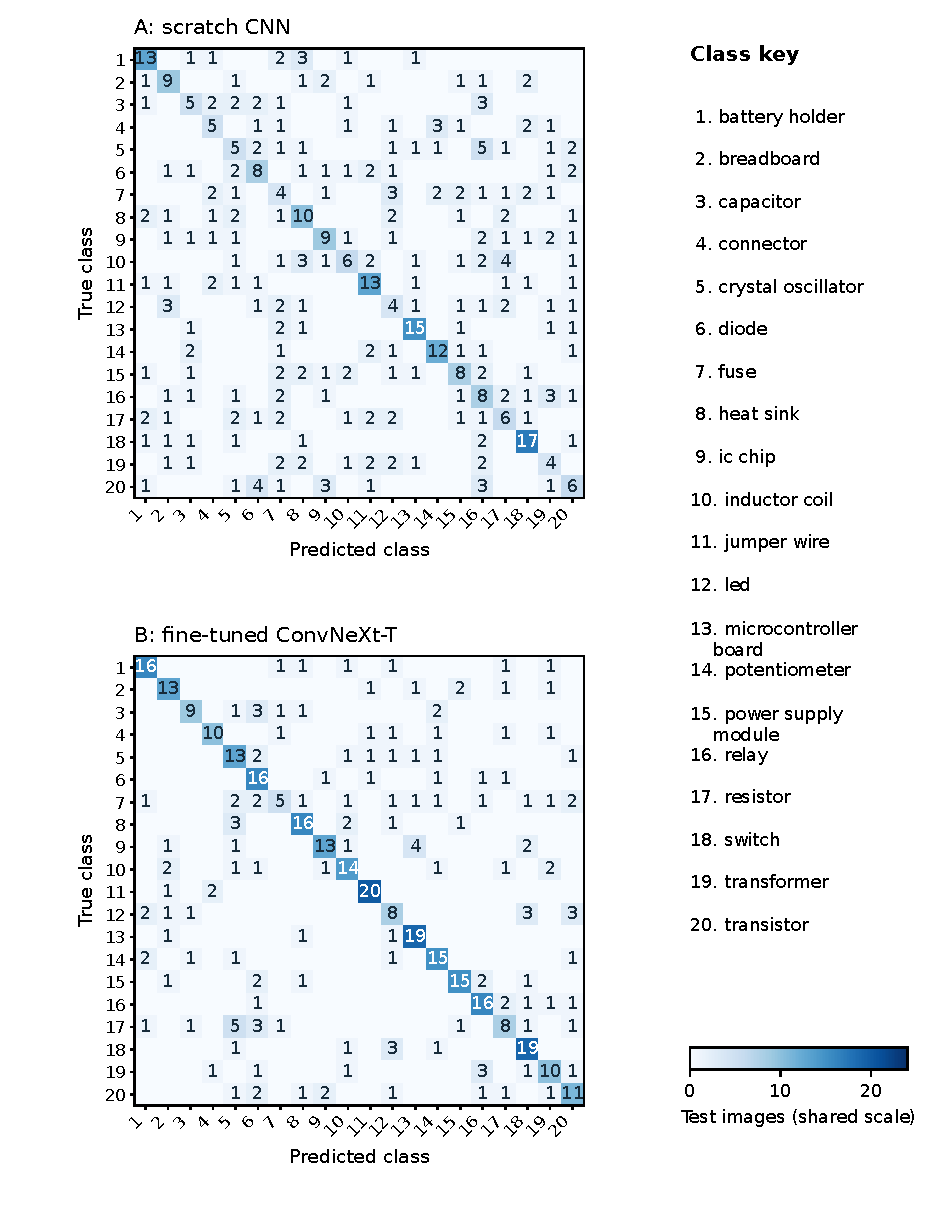
\includegraphics[width=\textwidth]{figures/confusion_AB.pdf}
\caption{Test confusion counts for A and B ($n=\nTest$). Numbered axes use the class key on the right;
rows are true classes and columns predictions. Zero cells are blank. The count scale is shared with \cref{fig:cmCD}.}
\label{fig:cm}
\end{figure}
\begin{figure}[p]
\centering
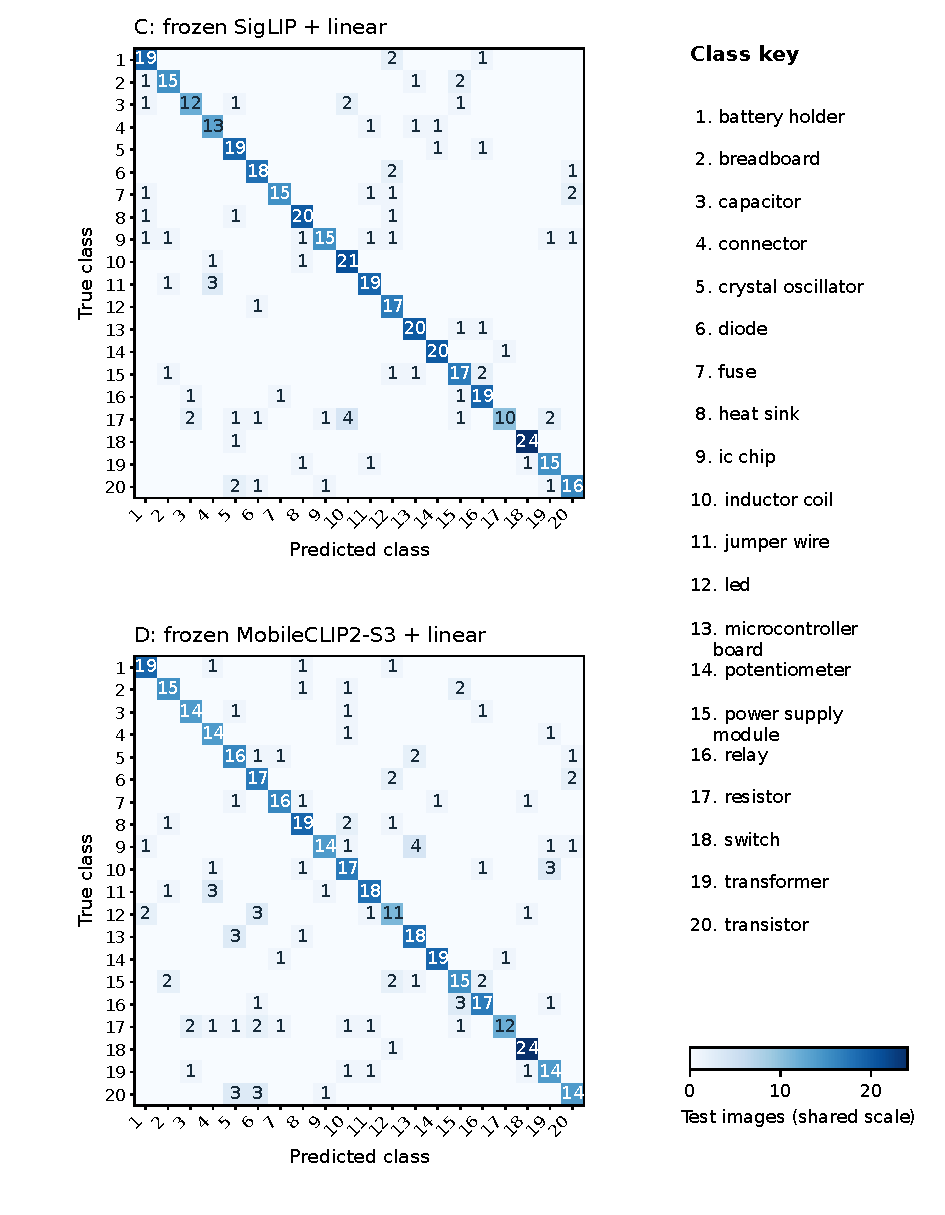
\includegraphics[width=\textwidth]{figures/confusion_CD.pdf}
\caption{Test confusion counts for C and D, with the same class key and count scale as \cref{fig:cm}.}
\label{fig:cmCD}
\end{figure}
\begin{figure}[p]
\centering
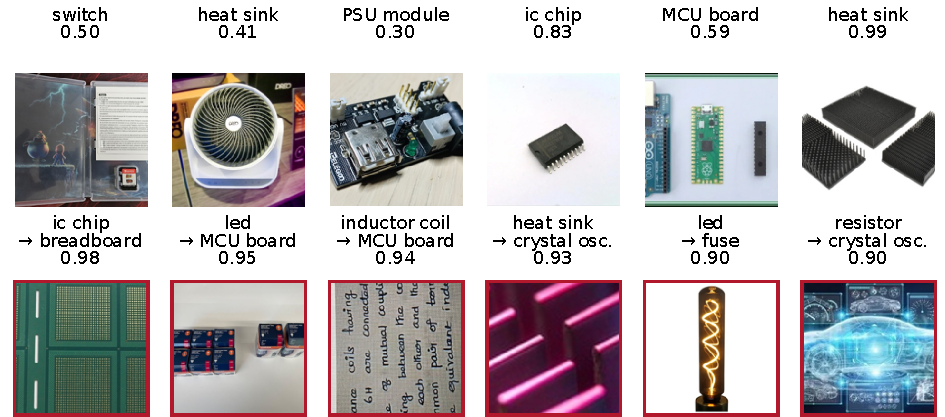
\includegraphics[width=\textwidth]{figures/gallery_A_scratch_cnn.pdf}
\par\medskip
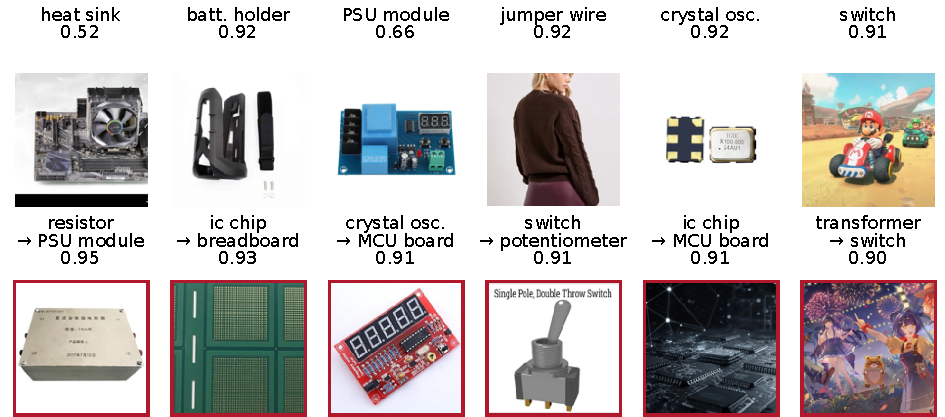
\includegraphics[width=\textwidth]{figures/gallery_B_convnext_tiny.pdf}
\caption{Model A (upper panel) and B (lower panel): six random correct predictions and six most confident errors
per model. Image selections, predictions and confidence values are unchanged; labels follow \cref{fig:galleries}.}
\label{fig:galleryAB}
\par\medskip
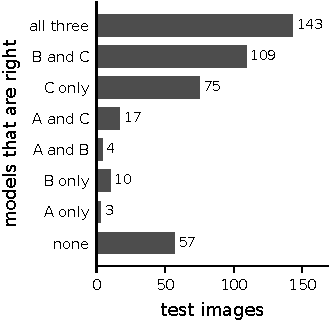
\includegraphics[width=0.43\textwidth]{fig09_agreement.pdf}
\caption{Test images by the subset of A, B and C that classifies them correctly (D excluded).}
\label{fig:agree}
\end{figure}
\begin{figure}[htbp]
\centering
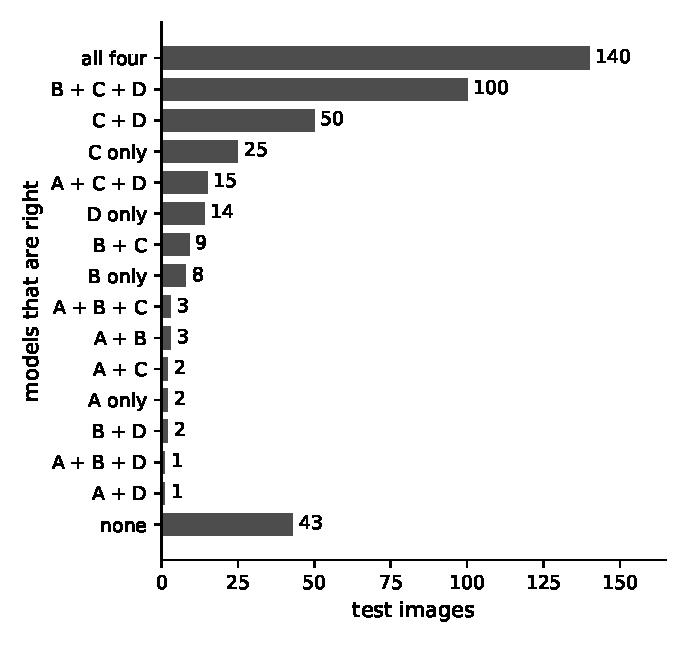
\includegraphics[width=0.5\textwidth]{figures/fig09_agreement_four_models.pdf}
\caption{Test images by the subset of all four models that classifies them correctly.}
\label{fig:agreeD}
\end{figure}
\FloatBarrier
\section{Additional dataset and training details}\label{app:extra}
\begin{table}[!htbp]
\centering\footnotesize\renewcommand{\arraystretch}{1.12}
\caption{Training settings: architecture and data.
Epochs are counted from 1. Optimisation and runtime settings continue below.}
\label{tab:hparams}
% generated by docs/itri626_report/make_tables.py -- do not edit by hand
\begin{tabularx}{\textwidth}{@{}>{\raggedright\arraybackslash}p{2.35cm}YVYVYVY@{}}
\toprule
 & \msq{A}\textbf{A}: scratch CNN & \msq{B}\textbf{B}: ConvNeXt-T (fine-tuned) & \msq{C}\textbf{C}: SigLIP ViT (frozen + linear) & \msq{D}\textbf{D}: MobileCLIP2-S3 (frozen + linear) \\
\midrule
\addlinespace[4pt]
\multicolumn{5}{@{}l}{\textsc{model}} \\
Model / variant & VGG-style CNN (scratch), width 32, 4 stages, dropout 0.3 & ConvNeXt-Tiny, stochastic depth (drop-path rate) 0.1 & ViT-So400m/14 (SigLIP), frozen; linear head (1,152 inputs, 20 outputs) & FastViT hybrid (MobileCLIP2-S3), frozen; linear head (3,072 inputs, 20 outputs) \\
Pretrained weights & none (He initialisation) & ImageNet-22k$\rightarrow$1k & WebLI & DFNDR-2B \\
Trainable / total params & 1,187,636 / 1,187,636 & 27,835,508 / 27,835,508 & 23,060 / 428,248,660 & 61,460 / 122,775,668 \\
\addlinespace[4pt]
\multicolumn{5}{@{}l}{\textsc{data and augmentation}} \\
Input size (px) & 160$\times$160 & 224$\times$224 & 384$\times$384 & 256$\times$256 \\
Augmentation (training only) & RandomResizedCrop (scale 0.35--1), h-flip 0.5, RandAugment (2,\,9), colour jitter 0.2 & RandomResizedCrop (scale 0.5--1), h-flip 0.5, RandAugment (2,\,9) & none (features of the evaluation crop) & none (features of the evaluation crop) \\
Class weights / sampling & none (uniform shuffling) & none (uniform shuffling) & none (uniform shuffling) & none (uniform shuffling) \\
Batch size; grad.\ accumulation & 64; none & 32; none & 256; none & 256; none \\
\bottomrule
\end{tabularx}

\end{table}
\begin{table}[!htbp]\ContinuedFloat
\centering\footnotesize\renewcommand{\arraystretch}{1.12}
\caption[]{Training settings (continued): optimisation, stopping and runtime. Times for C/D exclude feature extraction.}
\label{tab:hparamsTraining}
% generated by docs/itri626_report/make_tables.py -- do not edit by hand
\begin{tabularx}{\textwidth}{@{}>{\raggedright\arraybackslash}p{2.35cm}YVYVYVY@{}}
\toprule
 & \msq{A}\textbf{A}: scratch CNN & \msq{B}\textbf{B}: ConvNeXt-T (fine-tuned) & \msq{C}\textbf{C}: SigLIP ViT (frozen + linear) & \msq{D}\textbf{D}: MobileCLIP2-S3 (frozen + linear) \\
\midrule
\addlinespace[4pt]
\multicolumn{5}{@{}l}{\textsc{optimisation}} \\
Optimiser & AdamW, grad.\ clip 1.0 & AdamW, grad.\ clip 1.0 & AdamW & AdamW \\
Learning rate & 0.002 & 0.0002 & 0.001 & 0.001 \\
LR schedule & linear warm-up 5 epochs, cosine to 0 & head only in epoch 1, then all layers; warm-up 2 epochs, cosine to 0; layer-wise LR decay 0.8 & constant & constant \\
Weight decay & 0.05 (fixed) & 0.05 (fixed) & 0.0001 (grid on val., \cref{tab:wdgrid}) & 0.0001 (grid on val., \cref{tab:wdgridD}) \\
Loss & cross-entropy, label smoothing 0.1 & cross-entropy, label smoothing 0.1 & cross-entropy, label smoothing 0.0 & cross-entropy, label smoothing 0.0 \\
\addlinespace[4pt]
\multicolumn{5}{@{}l}{\textsc{regularisation and stopping}} \\
Early stopping & val.\ macro-F1, patience 40 & val.\ macro-F1, patience 6 & val.\ macro-F1, patience 20 & val.\ macro-F1, patience 20 \\
Epochs (max / run / best) & 200 / 200 / 184 & 20 / 20 / 19 & 200 / 34 / 14 & 200 / 31 / 11 \\
\addlinespace[4pt]
\multicolumn{5}{@{}l}{\textsc{runtime}} \\
Numerical precision & mixed fp16 & mixed fp16 & fp16 features, fp32 head & fp16 features, fp32 head \\
Random seed (training; split) & 0; 42 & 0; 42 & 0; 42 & 0; 42 \\
Training time & 390\,s (GPU) & 120\,s (GPU) & 1.7\,s for all 4 grid runs (CPU, cached features) & 2.4\,s for all 4 grid runs (CPU, cached features) \\
\bottomrule
\end{tabularx}

\end{table}

\Cref{tab:env} lists the software and hardware of the training run.
\begin{table}[!tbp]
\centering\footnotesize
\caption{Software and hardware of the training run of B and C; the final
run of A and the extraction and timing of D used a second machine (\cref{sec:software}).}
\label{tab:env}
\setlength{\tabcolsep}{4pt}
% generated by docs/itri626_report/make_tables.py -- do not edit by hand
\begin{tabularx}{\textwidth}{@{}lY@{}}
\toprule
Component & Version / specification \\
\midrule
Python & 3.12.14 \\
PyTorch / torchvision & 2.11.0+cu128 / 0.26.0+cu128 \\
timm (architectures and weights) & 1.0.30 \\
open\_clip\_torch & 3.3.0 \\
scikit-learn / NumPy / pandas & 1.9.1 / 2.5.4 / 3.0.6 \\
Pillow / matplotlib & 13.0.0 / 3.11.2 \\
ONNX / onnxruntime (deployment only) & 1.23.2 / 1.31.0 \\
CUDA (torch build) / cuDNN & 12.8 / 91900 \\
GPU & NVIDIA GeForce RTX 4060 Ti, 7.7\,GiB memory (compute capability 8.9) \\
NVIDIA driver & 615.71.09 \\
CPU / RAM & AMD Ryzen 7 8700F 8-Core Processor (16 logical cores) / 30.7\,GiB \\
Operating system & Linux-7.2.7-1-cachyos-x86\_64-with-glibc2.44 \\
Environment manager & uv (\texttt{pyproject.toml} + \texttt{uv.lock}) \\
\bottomrule
\end{tabularx}

\end{table}

\Cref{tab:curves} gives the state of each model at its selected epoch, \cref{tab:eff} model size and inference
time, \cref{fig:counts} the class distribution before and after cleaning and per split (the numbers are in
\cref{tab:dataset}), and \cref{tab:wdgrid} the weight-decay grid of \mC's head.

\begin{table}[htbp]
\centering\small
\caption{State at the selected (best validation macro-F1) epoch.
CE: cross-entropy.}
\label{tab:curves}
\footnotesize\setlength{\tabcolsep}{2.4pt}
% generated by docs/itri626_report/make_tables.py -- do not edit by hand
\begin{tabular}{@{}lrrrrrrr@{}}
\toprule
Model & Epochs run & Best epoch & Train acc. & Val.\ acc. & Val.\ macro-F1 & Train CE & Val.\ CE \\
\midrule
A: custom CNN & 120 & 106 & 0.586 & 0.339 & 0.329 & 1.471 & 2.361 \\
B: ConvNeXt-T FT & 20 & 19 & 0.904 & 0.618 & 0.617 & 0.542 & 1.431 \\
C: SigLIP ViT + linear & 34 & 14 & 0.986 & 0.803 & 0.801 & 0.139 & 0.759 \\
\bottomrule
\end{tabular}

\end{table}

\begin{table}[htbp]
\centering\small
\caption{Model size and inference time: forward pass of a preprocessed tensor
after warm-up, fp16 on the GPU, fp32 on 8 CPU threads, without JPEG decoding and resizing. C's and D's checkpoints hold only
the trained heads; the large backbone weights are additional. D was timed on an RTX 4070 Laptop, while A--C
were timed on the environment-table PC. D's tower was reparameterised for inference. MB follows the source files'
$2^{20}$-byte convention (MiB); these are not complete application download sizes.}
\label{tab:eff}
\footnotesize\setlength{\tabcolsep}{2.4pt}
% generated by docs/itri626_report/make_tables.py -- do not edit by hand
\begin{tabular}{@{}l S[table-format=3.2] S[table-format=8.0, group-minimum-digits=4] S[table-format=3.0] S[table-format=3.2] S[table-format=2.2] S[table-format=2.3] S[table-format=3.1]@{}}
\toprule
Model & {Params} & {Trainable} & {Input} & {Checkpoint} & {GPU, $b=1$} & {GPU, $b=32$} & {CPU, $b=1$} \\
 & {(M)} & {params} & {(px)} & {(MB)} & {(ms/img)} & {(ms/img)} & {(ms/img)} \\
\midrule
\msq{A}A: scratch CNN & 1.19 & 1187636 & 160 & 4.56 & 0.52 & 0.046 & 1.7 \\
\msq{B}B: ConvNeXt-T (fine-tuned) & 27.84 & 27835508 & 224 & 106.24 & 2.79 & 0.803 & 18.4 \\
\msq{C}C: SigLIP ViT (frozen + linear) & 428.25 & 23060 & 384 & 0.10 & 31.10 & 22.475 & 893.5 \\
\bottomrule
\end{tabular}

\end{table}


\begin{figure}[htbp]
\centering
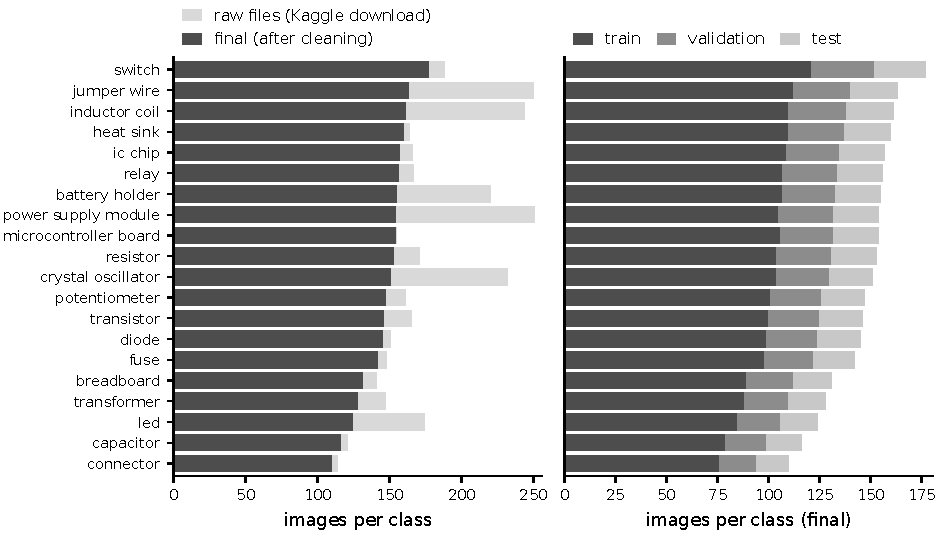
\includegraphics[width=\textwidth]{fig01_class_counts.pdf}
\caption{Left: images per class in the raw download (light) and after cleaning (dark). Right: the split of the cleaned
images into training, validation and test sets (\pctTrain\,/\,\pctVal\,/\,\pctTest\%).}
\label{fig:counts}
\end{figure}

\begin{table}[htbp]
\centering\small
\caption{Weight-decay selection for \mC's head on the validation set (learning rate $10^{-3}$, batch 256, at most
200 epochs, patience 20). The \nTies-way tie was broken by the pre-set
smallest-value rule. CE: cross-entropy.}
\label{tab:wdgrid}
% generated by docs/itri626_report/make_tables.py -- do not edit by hand
\begin{tabular}{@{}rrrrrrc@{}}
\toprule
Weight decay & Best epoch & Epochs run & Val.\ acc. & Val.\ macro-F1 & Val.\ CE & Selected \\
\midrule
\num{0.0001} & 14 & 34 & 0.8028 & 0.8011 & 0.7595 & yes \\
\num{0.001} & 14 & 34 & 0.8028 & 0.8011 & 0.7594 &  \\
\num{0.01} & 14 & 34 & 0.8028 & 0.8011 & 0.7594 &  \\
\num{0.1} & 21 & 41 & 0.8008 & 0.7999 & 0.7736 &  \\
\bottomrule
\end{tabular}

\end{table}

\begin{table}[htbp]
\centering\small
\caption{D's validation weight-decay grid: same learning rate, batch and stopping rule as C.
All four values tied on macro-F1; the pre-set smallest-value rule selected $10^{-4}$.}
\label{tab:wdgridD}
% generated by docs/itri626_report/make_tables.py -- do not edit by hand
\begin{tabular}{@{}rrrrr@{}}
\toprule
Weight decay & Best epoch & Val. acc. & Val. macro-F1 & Val. CE \\
\midrule
0.0001 & 11 & 0.775 & 0.772 & 0.900 \\
0.001 & 11 & 0.775 & 0.772 & 0.900 \\
0.01 & 11 & 0.775 & 0.772 & 0.899 \\
0.1 & 11 & 0.775 & 0.772 & 0.898 \\
\bottomrule
\end{tabular}

\end{table}
\begin{figure}[htbp]
\centering
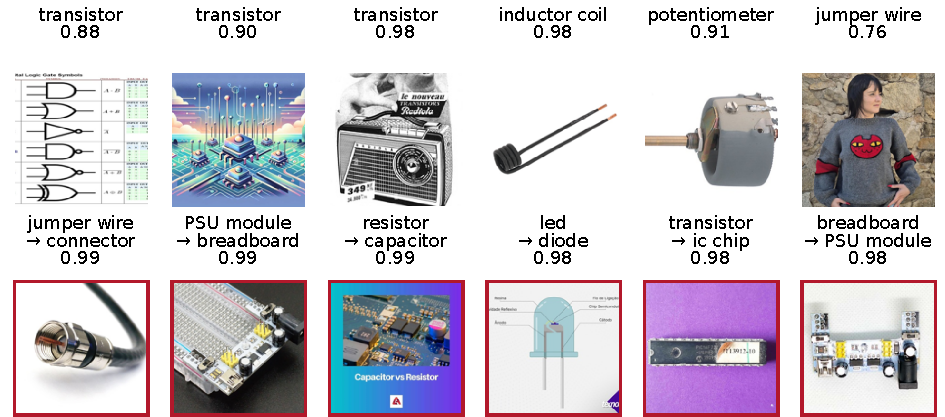
\includegraphics[width=\textwidth]{figures/gallery_D_mobileclip2_s3_linear.pdf}
\caption{D: six random correct predictions and six most confident errors; layout and abbreviations as in
\cref{fig:galleries}. Confidence is uncalibrated softmax probability.}
\label{fig:galleryD}
\end{figure}

\FloatBarrier\clearpage
\section{Supporting analysis}\label{app:benchmark}
This appendix details the supporting results summarised in \cref{sec:further}. In \cref{tab:benchmark}, fine-tuning used one fixed recipe per family, the probe is a
logistic regression on frozen features, and zero-shot uses the model's text encoder with class-name prompts and no
training.

\begin{table}[!tbp]
\centering\footnotesize
\caption{Scratch-CNN improvement study. Development: grouped 5-fold macro-F1 (mean $\pm$ SD over folds). Test
and holdout: one training run on the fixed split, scored once. The
120-epoch row is the model A of the previous build of this report; R2 is the deployed model of \cref{tab:test}.}
\label{tab:improveA}
\setlength{\tabcolsep}{1.9pt}
% generated by docs/itri626_report/make_tables.py -- do not edit by hand
\begin{tabular}{@{}lcccccc@{}}
\toprule
Recipe & Epochs & Dev.\ 5-fold macro-F1 & Test macro-F1 & Test acc. & Holdout macro-F1 & Holdout acc. \\
\midrule
A, previous build & 120 & 0.355 $\pm$ 0.015 & 0.336 & 0.354 & -- & -- \\
\textbf{A, this report} & 200 & 0.390 $\pm$ 0.007 & 0.392 & 0.400 & 0.257 & 0.283 \\
\addlinespace[2pt]
Deployed SigLIP model (R2) & -- & -- & 0.834 & 0.837 & 0.816 & 0.821 \\
\bottomrule
\end{tabular}

\end{table}

\textbf{Eleven-family benchmark.} Grouped 5-fold cross-validation on the 2,512 development images
(\cref{tab:benchmark}) reproduces the ordering: scratch CNN \bmScratch macro-F1, ConvNeXt-T
fine-tuned \bmConvnext, frozen SigLIP So400m probe \bmProbeSiglip. All six ImageNet-pretrained fine-tunes lie between
\bmImagenetLo and \bmImagenetHi, SigLIP zero-shot classification without training (\bmZeroSiglip) beats all of them,
and partial fine-tuning of the SigLIP backbone (\bmPartial, three folds) did not beat the frozen probe.


\textbf{Leakage of the original split.} Under the dataset's original file-level split, \leakRows of the \leakEval
deduplicated development images that it places in validation or test (\leakPct\%) also have a copy in its training
part (our own test images are excluded; \cref{sec:split} counts raw file entries instead), which inflates three linear probes by \inflSiglip
(SigLIP), \inflConvnext (ConvNeXt-T) and \inflResnet (ResNet-50) points in the recorded leakage simulation.
Weaker models gain most, so leakage also compresses the gaps between models. 

\textbf{Out-of-source test and deployment.} The deployed model (R2) was tested once on \whN Wikimedia Commons
photographs collected after it was frozen: \whAcc accuracy and \whFone macro-F1, close
to its in-distribution result. Its weakest classes there are \cls{led} (recall \whRecLed; \whCmLedDiode errors to
\cls{diode}), \cls{switch} (\whRecSwitch; real switches predicted \cls{ic chip} \whCmSwIc times, a consequence of the
console-dominated training class) and \cls{transformer} (\whRecTrf; \whCmTrfInd errors to \cls{inductor coil}). It is
exported to ONNX for an OpenCV demo and a Rust desktop application.


\textbf{Efficiency study and packaged models.} Model selection in the efficiency study used five grouped development folds, rather than test results. With the fused recipe and the same RTX 4070 Laptop,
fp16 ONNX Runtime CUDA batch-1 latency was 31.9 ms for SigLIP at 384 px, 20.4 ms at 308 px and 8.9 ms for
MobileCLIP2-S3. Their development OOF macro-F1 values were 0.840, 0.822 and 0.801. The 308 px row measures the
Fast-resolution tower at fp16; it is not an INT8 TensorRT measurement. These runtime measurements differ from
\cref{tab:eff}'s PyTorch timings and exclude image decoding and resizing.
The packaged Small model subsequently scored 0.806 accuracy and 0.802 macro-F1 once on the 418 test rows. It is R3 here; its 0.55 abstention threshold and fitted fusion
must not be attributed to D. No new test evaluation was performed for this report revision.

\begin{figure}[htbp]
\centering
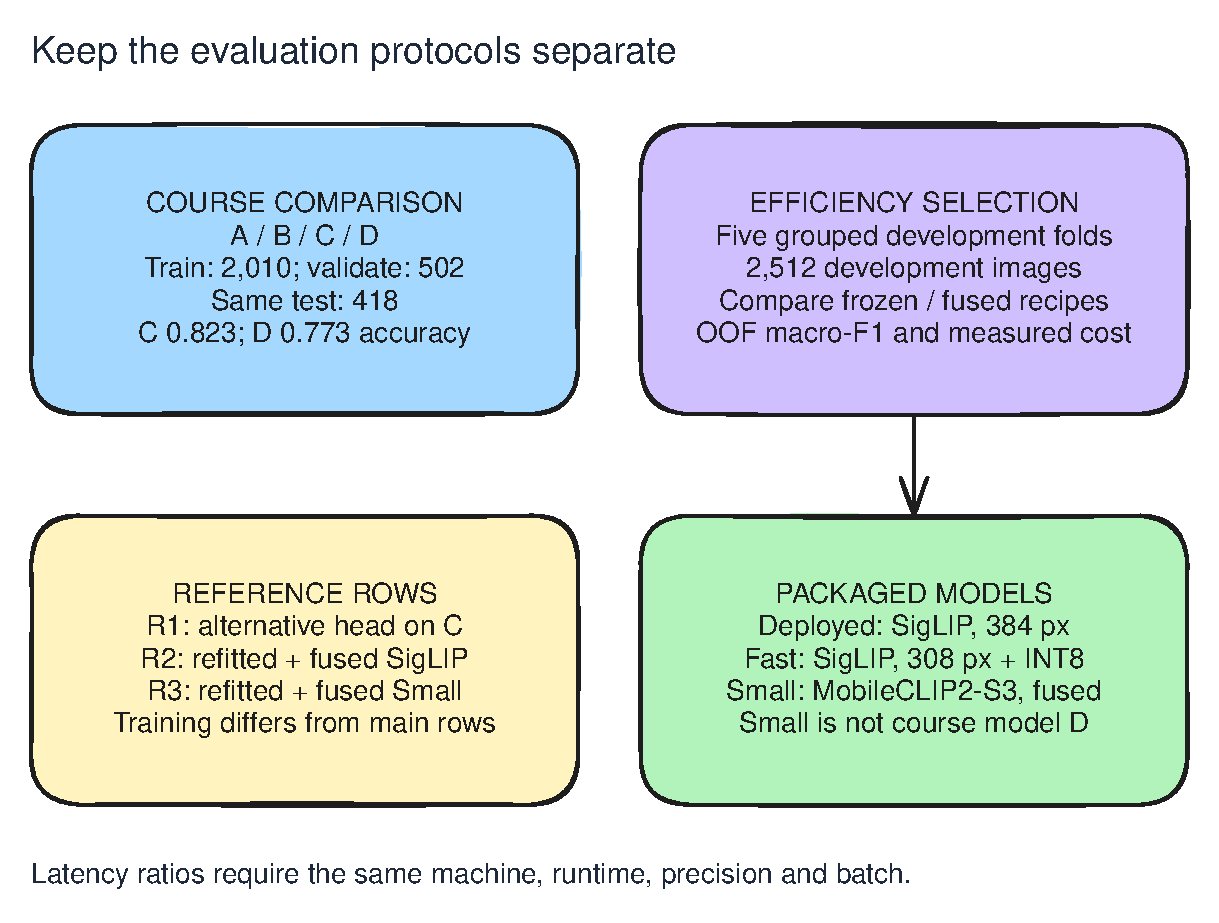
\includegraphics[width=0.92\textwidth]{diagrams/protocols.pdf}
\caption{Three distinct uses of the data: matched course models, development-fold efficiency selection and
refitted deployment references. OOF means out-of-fold. Excalidraw sources accompany the exports.}
\label{fig:protocols}
\end{figure}

\begin{table}[htbp]
\centering\small
\caption{Supporting benchmark: grouped 5-fold CV macro-F1 (mean $\pm$ SD over folds) on the development set. $^{\dagger}$Three folds only. C shares the SigLIP backbone with the probe column; the head-fitting procedure differs.}
\label{tab:benchmark}
\setlength{\tabcolsep}{1.9pt}
% generated by docs/itri626_report/make_tables.py -- do not edit by hand
\begin{tabular}{@{}lccc@{}}
\toprule
Family (variant) & Fine-tune & Frozen linear probe & Zero-shot \\
\midrule
Classical: HOG + colour histogram + SVM & \multicolumn{3}{c}{0.206 $\pm$ 0.017 (classical pipeline)} \\
Scratch CNN (model A's network, 120-epoch recipe) & 0.355 $\pm$ 0.015 & -- & -- \\
ResNet-50 & 0.580 $\pm$ 0.012 & 0.515 $\pm$ 0.018 & -- \\
MobileNetV3-L & 0.547 $\pm$ 0.016 & -- & -- \\
EfficientNetV2-S & 0.608 $\pm$ 0.024 & -- & -- \\
ConvNeXt-T (as model B) & 0.641 $\pm$ 0.034 & 0.593 $\pm$ 0.021 & -- \\
ViT-B/16 (AugReg) & 0.654 $\pm$ 0.032 & -- & -- \\
Swin-T & 0.639 $\pm$ 0.034 & -- & -- \\
DINOv2 (FT: ViT-B/14; probe: ViT-L/14) & 0.668 $\pm$ 0.024 & 0.667 $\pm$ 0.019 & -- \\
CLIP (FT: ViT-B/16; others: ViT-L/14@336) & 0.702 $\pm$ 0.017 & 0.721 $\pm$ 0.019 & 0.609 $\pm$ 0.029 \\
SigLIP So400m/14@384 (backbone of C) & 0.812 $\pm$ 0.023$^{\dagger}$ & 0.824 $\pm$ 0.012 & 0.776 $\pm$ 0.018 \\
\bottomrule
\end{tabular}

\end{table}

\FloatBarrier\clearpage
\textbf{Detailed limitations of the comparison.}
\begin{enumerate}[leftmargin=*]
\item \textbf{One split, one training seed.} With about 21 test images per class, one image can materially change a per-class F1, and the precision of an accuracy difference depends on the models' paired errors; no fixed significance threshold applies. The cross-validation benchmark
gives the same ordering.
\item \textbf{Noisy labels and scope.} Labels are unreviewed search terms and \pctOOD\% of the images are flagged as
possibly off-topic (by an automated screen that no person verified). Measured accuracy need not represent
performance on clean photographs. Because no person checked the test labels either, per-class scores for homonym
classes (\cls{switch}, \cls{transformer}) partly measure the scrape rather than the model.
\item \textbf{Screen and model share a lineage.} The off-topic flags come from a CLIP model, a relative of C's
SigLIP encoder, so the flagged/unflagged comparison in \cref{sec:errors} may favour C.
\item \textbf{Residual near-duplicates.} The near-duplicate rule (pHash and CLIP thresholds) can miss heavily edited
copies, so some train--test similarity may remain.
\item \textbf{Unequal pretraining and budgets.} C's backbone was trained on far more data than B's, so the comparison
measures model and pretraining together. The budgets of A and B were fixed by earlier cross-validation, not tuned
exhaustively. A was then trained to convergence, and the study of \cref{sec:improveA} found no further recipe gain,
so the observed gap of \diffCA points to C persists under the tested budgets.
\item \textbf{D's asymmetries.} D uses a different crop fraction and was timed on a second PC; the
same-PC C-tower anchor is reported separately. Its weights have research-use restrictions under the Apple Machine Learning Research Model License; commercial suitability is not established.
\item \textbf{Cost.} C has \paramsMC million parameters and needs about \cpuMsC\,ms per image on a CPU, which rules it
out for microcontrollers or real-time video without a GPU.
\end{enumerate}

\FloatBarrier\clearpage
\section{Reproduction}\label{app:repro}
The \href{https://github.com/Vaperizer2/626-Project}{project repository} contains the source code, executed
comparison notebook, fixed split assignments, committed predictions and metrics, figure sources and build instructions.
The repository is private; access requires a collaborator invitation. Raw images are obtained separately from the
Kaggle source cited in \cref{sec:source}. Rebuilding the cleaned dataset should reproduce \nRows images and manifest
fingerprint \fingerprint.

Python dependencies are pinned by the committed lockfile and managed with uv. The report tables and number macros
are generated from committed results, and the PDF is compiled with LaTeX. Rebuilding the report neither trains
models nor scores images. The comparison notebook also defaults to displaying recorded results without retraining.

The accompanying records identify the sources of the cleaning ablation, label audit, off-topic flags, confidence
thresholds and broader benchmark. Each reported number is linked to its source in a machine-readable provenance
register. Wikimedia photograph credits are retained in the attribution register.

Training and data-rebuild procedures are provided for historical reproducibility. Both recorded holdouts are spent;
use development or synthetic inputs for routine checks. Model A was imported from the improvement study's fold-0 run
rather than retrained for this report.

\end{document}
